\chapter{Results}

\section{Deuteron photodisintegraion}

    \subsection{Cross section}
    \label{cross_results}

    In this section I will show the results of my calculation starting from the
    deuteron photodisintegration process. One of the most
    studying observable is obviously cross section. There is
    a number of papers which present 
    measurement results for both differential and total cross section
    \cite{BOSMAN1979,ARENDS1984,Skopik1974, Moreh1989, Birenbaum1985, Bernabei1986, rachek2007,Ying_Experiment_Deut, DeSanctis_Experiment_Deut} so it is convenient 
    to prepare a theoretical predictions in order to compare 
    it with experimental results.

    On the Fig.~\ref{TOTAL_CROSS_small} and Fig.~\ref{TOTAL_CROSS} 
    I present predictions for the
    total cross section $\sigma_{tot}~[\mu\text{b}]$ which I obtained
    using the chiral potential at the order N$^4$LO+ and with 
    the cutoff parameter $\Lambda=450$~MeV (my best predictions).
    Looking at Fig.~\ref{TOTAL_CROSS_small}, we can see that at low photon energies
    (below 50 MeV) my predictions which include 2N contributions
    using Siegert approach, describe experimental results quite well.
    We can suppose that the difference with experimental data may come from 
    the statistical uncertainty of  the data itself, as my predictions
    are often in between the data from different sources.
    Moreover even at such low energies the 1N current is clearly not enough
    to describe this observable as dashed pink line has much lower values and
    the difference becomes even larger with larger photon's energies. 

    Having look at the higher energies (above 50~MeV, Fig.~\ref{TOTAL_CROSS})
    we can notice that the difference with experimental data is not only 
    quantitative, but also qualitative.  There is a peak around 300~MeV
    in the experimental data from \cite{Bernabei1986} which is not
    reflected in my predictions. The reason of such discrepancy 
    is most likely coming from the relativistic effects
    which I do not take into account. At higher energies their contribution
    becomes larger and here we observe a clear justification of such a lack.
    It is also confirmed by the calculations in \cite{ArenhovelPhotodisint1991}
    where authors present predictions obtained with and without including
    relativistic effects and such a peak appears in the latter case. 
    
    Nevertheless my main goal is to describe deuteron photodisintegration at low energies and predictions seem to be well describing experimental data at
    $E_\gamma \lesssim 50$~MeV. The higher energies region is presented in order
    to investigate how far the predictions are from experimental results and 
    what can be improved in the future (e.g. include relativistic part). 
    
    \begin{figure}[h]
        \begin{center}
        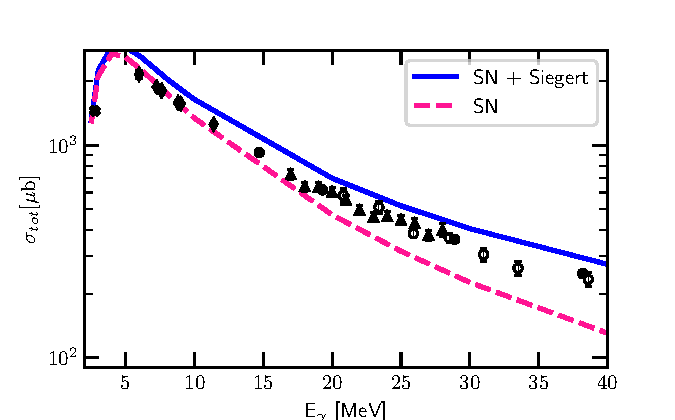
\includegraphics[width=0.75\textwidth]{Figures_python/TOTAL_CROSSSECTION_SMALL_REGION.pdf}
        \end{center}
        \caption{The same as on the Fig.~\ref{TOTAL_CROSS} but for the energy range 2.5 - 40 MeV.
        }
        \label{TOTAL_CROSS_small}
    \end{figure}

    
    \begin{figure}[h]
        \begin{center}
        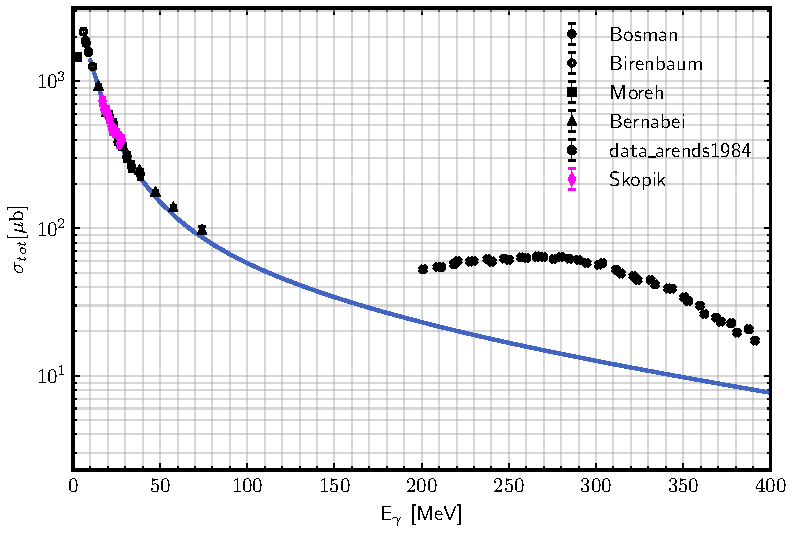
\includegraphics[width=0.75\textwidth]{Figures_python/TOTAL_CROSSSECTION.pdf}
        \end{center}
        \caption{Total cross section as a function of the photon's energy E$_\gamma$.
        Solid blue line presents results obtained with SN+Siegert 
        and dashed pink line - with only SN current.
        The experimental data are from \cite{Bernabei1986} (black filled circles),
        \cite{BOSMAN1979} (empty circles),
        \cite{ARENDS1984} (squares),
        \cite{Skopik1974} (triangles),
        \cite{Moreh1989} (cross "X") and
        \cite{Birenbaum1985} (dimonds).
        }
        \label{TOTAL_CROSS}
    \end{figure}
    
        
    {\color{red} Maybe better reorganize figures, combine similar figures for different energies in one?}

    Figures \ref{Diff_cross_order} - \ref{Diff_cross_cutoff} show my predictions for the differential cross section
    $\frac{d\sigma}{d\Omega}$, where each subfigure 
    presents results obtained using different values of the photon energy:
    30, 100 and 140~MeV. 
    % They all are organized in a similar way: the left panel
    % presents predictions obtained using SMS potential at different chiral orders (from LO to N$^4$LO+)
    % with cutoff parameter $L = 450$~MeV,
    % the middle panel includes the truncation error's bands (described in Sec. \ref{sec:deut_bound})
    % for each chiral order starting
    % from NLO. And the right panel shows predictions obtained with different values of the
    % cutoff parameter at the chiral order N$^4$LO+.
    Fig.~\ref{Diff_cross_order} shows the predictions obtained using 
    different chiral orders (from LO to N$^4$LO+) and with $\Lambda=450$~MeV.
    Comparing the best predictions (N$^4$LO+, $\Lambda=450$~MeV) for each
    subfigure, we can once more 
    conclude that the higher photon's energy is, the larger is 
    difference between the theoretical predictions and experimental 
    measurements. At $E_\gamma = 30$~MeV (top pane) my predictions
    almost perfectly match the data and the difference is almost always
    within the experimental uncertainties. Going to the energy 100~MeV (middle subfigure)
    the descriptions seems not to be such good: theoretical
    predictions match experimental data qualitatively, but
    the gap in the angles range ($60^{\circ} < \theta_p < 130^{\circ}$) 
    is around 30\% ({\color{red} check the value!}).
    Looking at the bottom figure, it is even hard to say about 
    good qualitative description: the general trend of the
    angular dependance is presented, but still the predictions are 
    far from experimental values.
    In addition, figures for each energy confirm the convergence 
    of the predictions with respect to the chiral order.
    We see that the curves at LO are far from both experimental 
    data and the best potential's predictions (N$^4$LO+) and
    the higher is photon's energy, the larger is this
    difference. With each subsequent chiral order, the 
    curves are more closer to each other and the difference
    between N$^4$LO and N$^4$LO+ is hardly visible at current scale.
    So I can conclude that predictions are converged and 
    further chiral orders would rather not bring large contribution 
    to the cross section values. What may be helpful
    for a better data description is a 2N current 
    and relativistic correction, mentioned earlier.

    The Fig.~\ref{Diff_cross_truncation} 
    presents theoretical (truncation) uncertainties and it once more
    confirms that for the regarded nuclear reaction chiral order
    N$^4$LO+ is able to produce converged predictions: 
    the black band is hardly visible for the $E_\gamma=30$~MeV 
    and is also quite narrow for larger energies. 
    The difference with experimental data is rather systematic 
    and is independent on the chiral order. 

    Fig.~\ref{Diff_cross_cutoff} presents a cutoff dependency
    of my predictions. The ideal case is when the dependency is so weak that
    the choice of the parameter $\Lambda$ would not make large 
    changes. In practice the choice of this parameter can be 
    important as it makes a noticeable difference in predictions.
    
    On the top figure the cutoff dependance is so weak,
    that, in fact, all the lines (for different $\Lambda$ values)
    overlap each other and we cannot distinguish them with the naked eye.
    Nevertheless, with increasing photon's energy to 100 and 140~MeV 
    (middle and bottom figures) the spread becomes larger. 
    Although the spread is visible, it is not so large and even for 140~MeV
    it is within 12\%. 

    On the Fig.~\ref{Cutoff_dep} we saw that the total
    cross section for the same energies has the cutoff spread
    around 4.5\% for 100~MeV and 8\% for 140~MeV. For 30~MeV it is below 1\%.  
    

    \begin{figure}[h]
        \begin{center}
        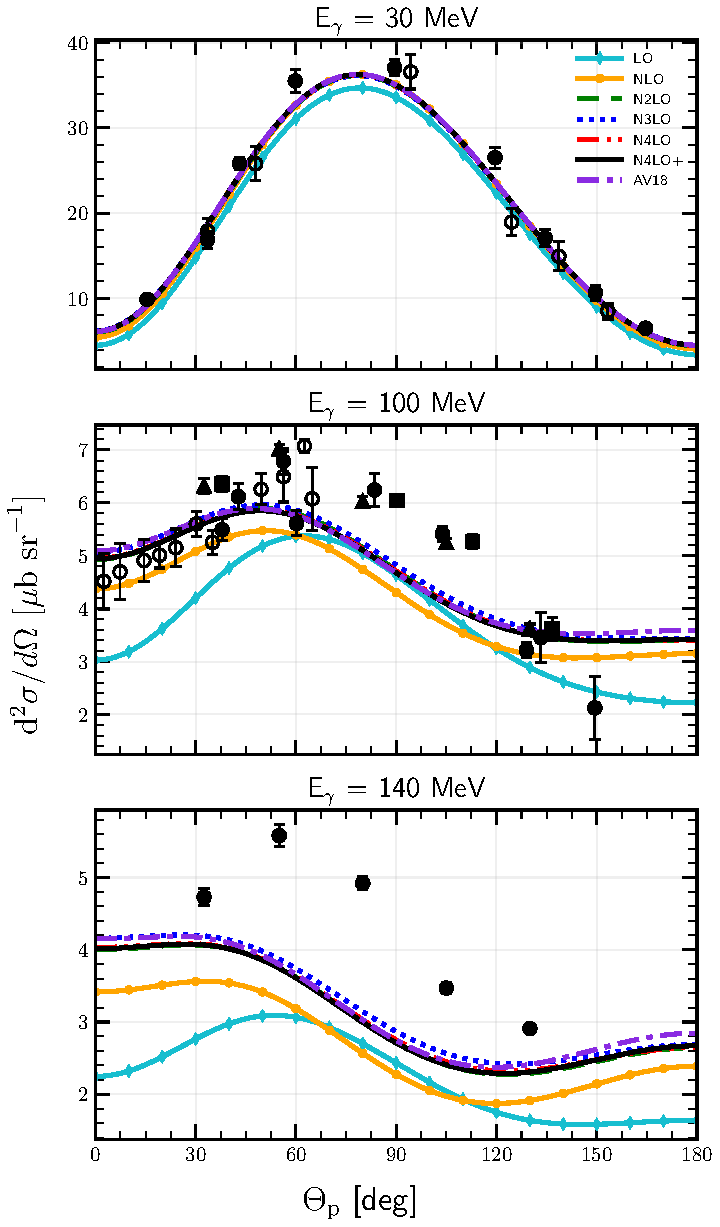
\includegraphics[width=0.7\textwidth]{Figures_python/CROSS2_order_vert.pdf}
        \end{center}
        \caption{Differential cross section as a function of the outgoing proton angle in the center of mass frame 
        for the photon's energy 30 MeV (top), 100 MeV (middle) and 140 MeV (bottom). Results are obtained using potential
        with different chiral orders (from LO to N$^4$LO+) with cutoff parameter $\Lambda=450$~MeV.
        For the sake of comparison, predictions obtained with AV18 potential are on both figures as well.
        Data points (filled and empty circles) are from \cite{Ying_Experiment_Deut}
        for (30 and 100 meV)
        and \cite{DeSanctis_Experiment_Deut} (for energy 140 MeV).}
        \label{Diff_cross_order}
    \end{figure}


    \begin{figure}[h]
        \centering
        \begin{subfigure}[b]{0.46\textwidth}
            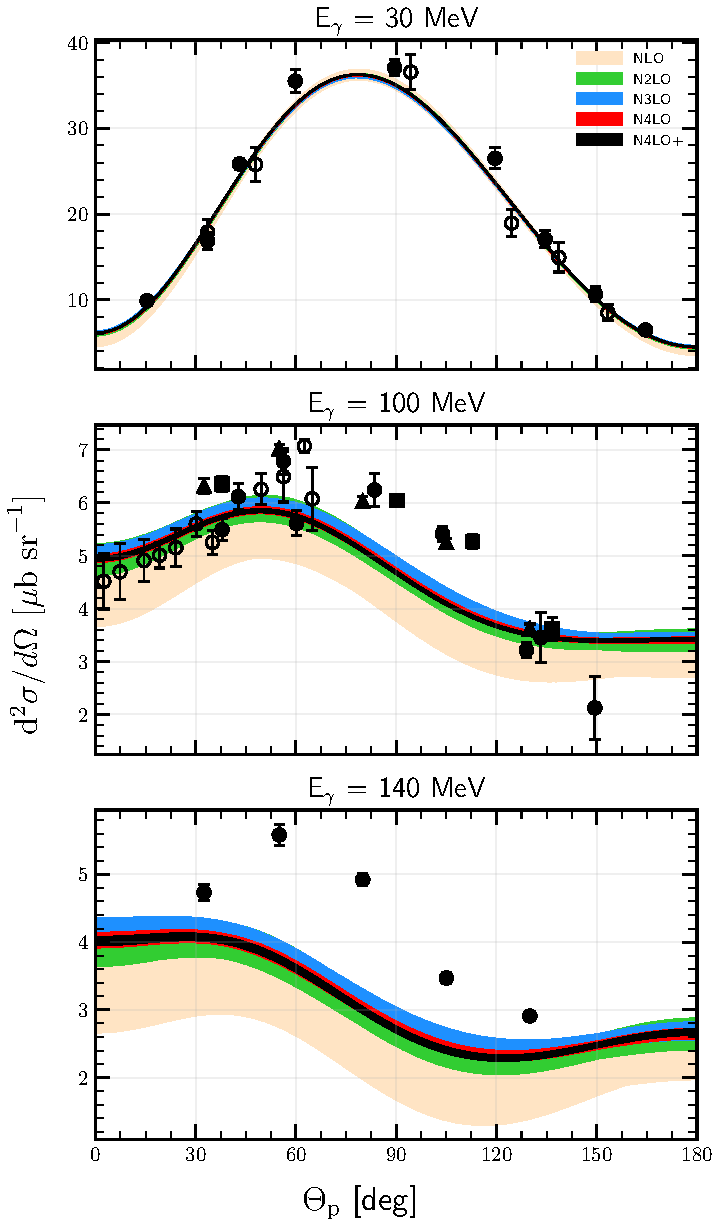
\includegraphics[width=\textwidth]{Figures_python/CROSS2_truncation_vert.pdf}
            \caption{Truncation error bands}
            \label{Diff_cross_truncation}
        \end{subfigure}
        \begin{subfigure}[b]{0.46\textwidth}
            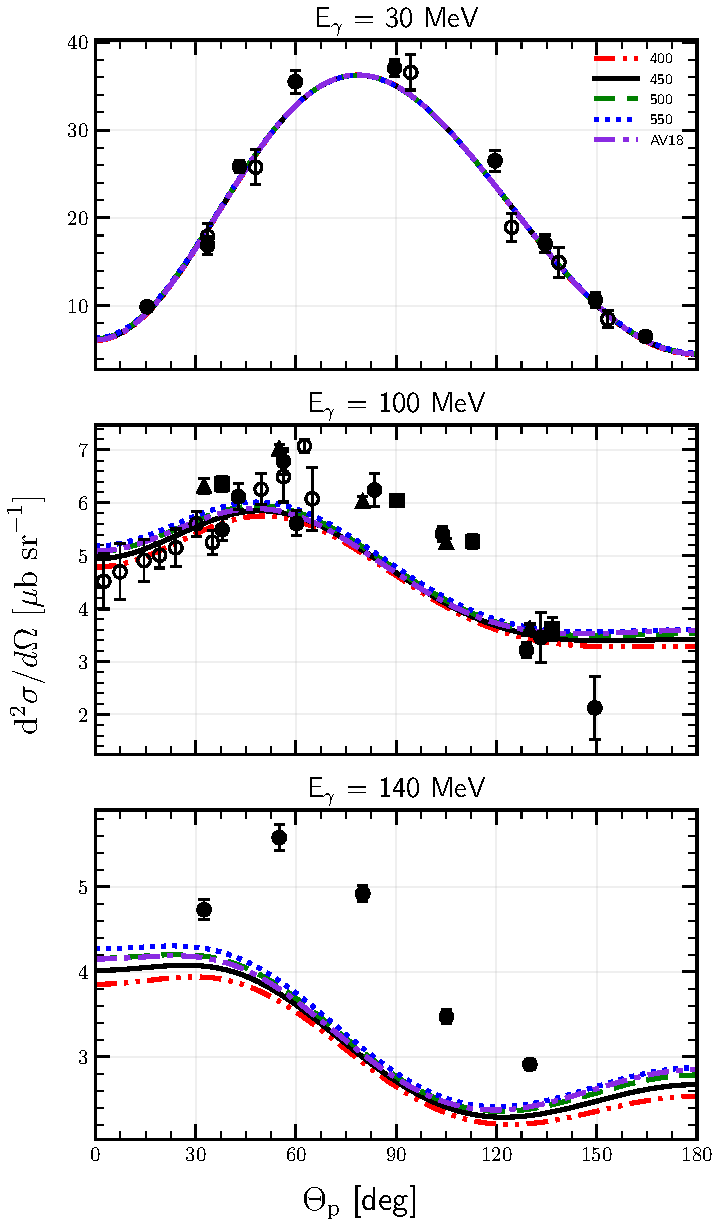
\includegraphics[width=\textwidth]{Figures_python/CROSS2_cutoff_vert.pdf}
            \caption{Cutoff dependance}
            \label{Diff_cross_cutoff}
        \end{subfigure}
        \caption{Differential cross section as a function of the outgoing proton angle in the center of mass frame 
        for the photon's energy is 30 MeV (top row), 100 MeV (middle row) and 140 MeV (bottom row).
        Figure {\bf(a)} presents a truncation error bands for each energy in corresponant row. 
        Results are obtained using potential with different chiral orders (from NLO to N$^4$LO+) 
        with cutoff parameter $\Lambda=450$~MeV.
        Figure {\bf (b)} shows predictions obtained using different values of the cutoff parameter $\Lambda$
        (double-dotted-dashed red line presents results obtaining with 
        a cutoff values $\Lambda=400$~MeV, solid black line - 450~MeV, dashed green line - 500~MeV
        and dotted blues line - 550~MeV) and chiral potential N$^4$LO+. 
        Data points (filled and empty circles) are from \cite{Ying_Experiment_Deut}
        for (30 and 100 meV)
        and \cite{DeSanctis_Experiment_Deut} (for 140~MeV).}
    \end{figure}


    % \begin{figure}[h]
    %     \begin{center}
    %     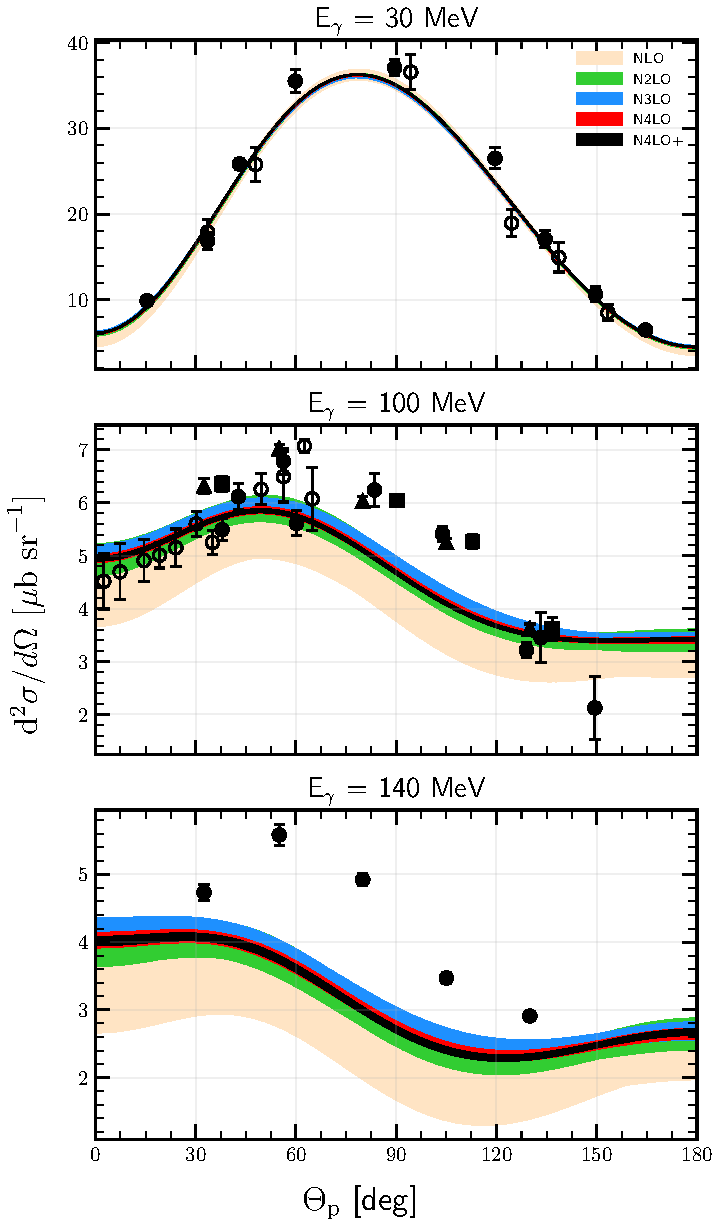
\includegraphics[width=0.7\textwidth]{Figures_python/CROSS2_truncation_vert.pdf}
    %     \end{center}
    %     \caption{Truncation error's bands for the differential cross section 
    %     as a function of the outgoing proton angle in the center of mass frame 
    %     The photon's energy is 30 MeV (top pane), 100 MeV (middle) and 140 MeV (bottom). Results are obtained using potential
    %     with different chiral orders (from LO to N$^4$LO+) with cutoff parameter $\Lambda=450$~MeV.
    %     Data points (filled and empty circles) are from \cite{Ying_Experiment_Deut}
    %     for (30 and 100 meV)
    %     and \cite{DeSanctis_Experiment_Deut} (for energy 140 MeV).}
    %     \label{Diff_cross_truncation}
    % \end{figure}

    

    % \begin{figure}[h]
    %     \begin{center}
    %     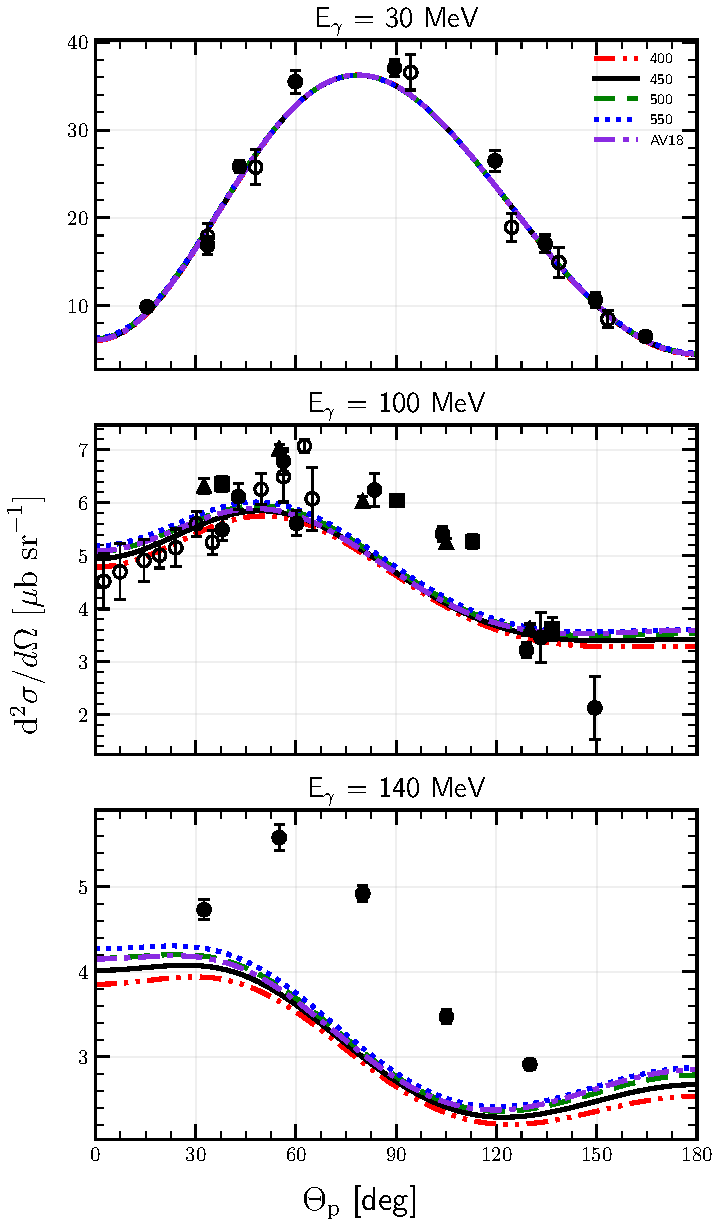
\includegraphics[width=0.7\textwidth]{Figures_python/CROSS2_cutoff_vert.pdf}
    %     \end{center}
    %     \caption{Differential cross section as a function of the outgoing proton angle in the center of mass frame 
    %     for the photon's energy is 30 MeV (top pane), 100 MeV (middle) and 140 MeV (bottom). 
    %     The double-dotted-dashed red line presents results obtaining with 
    %     a cutoff values $\Lambda=400$~MeV, solid black line - 450~MeV, dashed green line - 500~MeV
    % and dotted blues line - 550~MeV.
    %     For the sake of comparison, predictions obtained with AV18 potential (purple dotted-dashed line).
    %     Data points (filled and empty circles) are from \cite{Ying_Experiment_Deut}
    %     for (30 and 100 meV)
    %     and \cite{DeSanctis_Experiment_Deut} (for energy 140 MeV).}
    %     \label{Diff_cross_cutoff}
    % \end{figure}

    
        
    % \begin{figure}[h]
    %     \begin{center}
    %     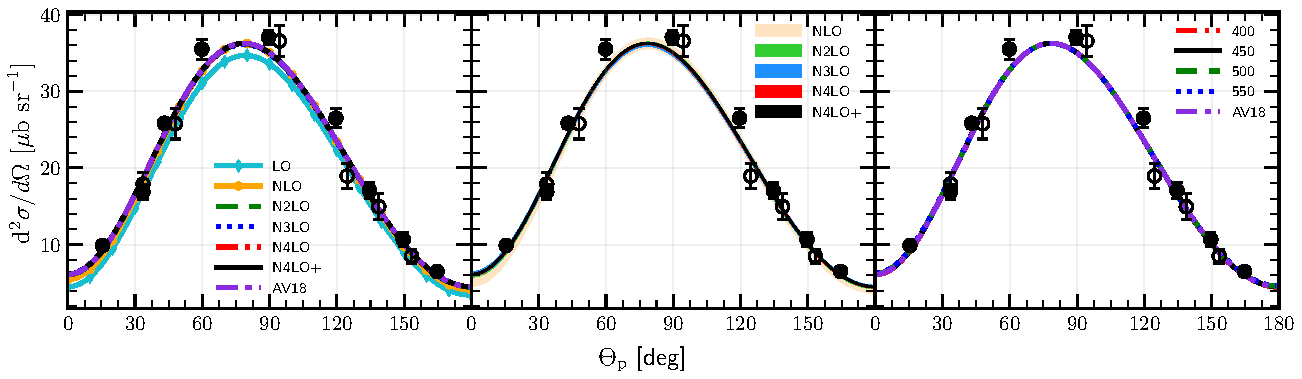
\includegraphics[width=0.95\textwidth]{Figures_python/CROSS2_30mev.pdf}
    %     \end{center}
    %     \caption{Differential cross section as a function of the outgoing proton angle in the center of mass frame 
    %     for the photon's energy 30 MeV. Left figure presents results obtained using potential
    %     with different chiral orders (from LO to N$^4$LO+) with cutoff parameter $\Lambda=450$~MeV
    %     whereas right figure presents a cutoff dependency and chiral potential N$^4$LO+ was used in all cases.
    %     For the sake of comparison, predictions obtained with AV18 potential are on both figures as well.
    %     Data points (filled and empty circles) are from \cite{Ying_Experiment_Deut}.}
    %     \label{CROSS_30}
    % \end{figure}
        

    % \begin{figure}[h]
    %     \begin{center}
    %     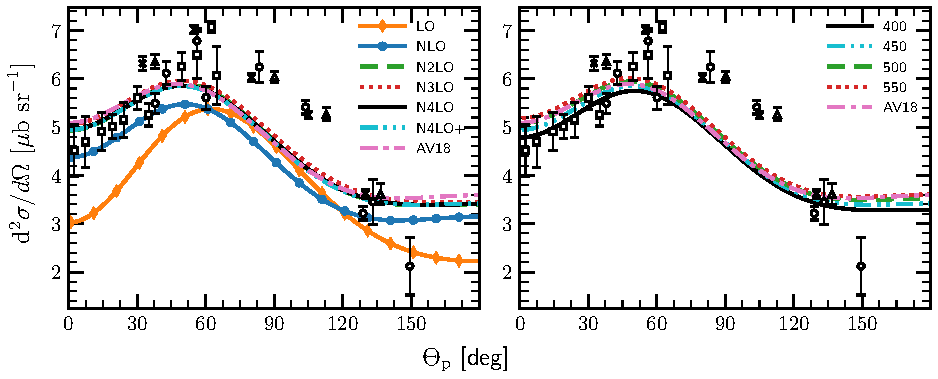
\includegraphics[width=0.95\textwidth]{Figures_python/CROSS2_100mev.pdf}
    %     \end{center}
    %     \caption{The same as on the Fig.~\ref{CROSS_30} but for the photon's energy E$_\gamma$=100~MeV.
    %     All experimental data points (filled and empty circles, squares and triangles) are from \cite{Ying_Experiment_Deut}.}
    %     \label{CROSS_100}
    % \end{figure}

    % \begin{figure}[h]
    %     \begin{center}
    %     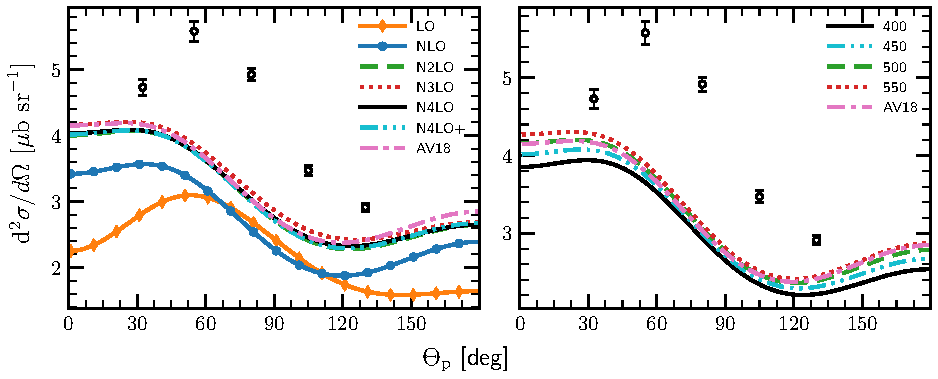
\includegraphics[width=0.95\textwidth]{Figures_python/CROSS2_140mev.pdf}
    %     \end{center}
    %     \caption{The same as on the Fig.~\ref{CROSS_30} but for the photon's energy E$_\gamma$=140~MeV.
    %     The data are from \cite{DeSanctis_Experiment_Deut}.}
    %     \label{CROSS_140}
    % \end{figure}
    \clearpage

    \subsection{Polarisation observables}
    \label{tensor_results}

    In this subsection I will present my predictions for 
    selected polarisation observables.
    I start with deuteron analyzing power $T_{20}$, $T_{21}$ and $T_{22}$,
    which according to \cite{ArenhovelPhotodisint1991} are defined as:
    
    \begin{equation}
        T_{2i} (\theta) = \frac{(2 - \delta_{i0}) \Re V_{2i}}{V_{00}}, i=0,1,2
    \end{equation}

    On the Figures \ref{T20_100_vert}, \ref{T21_100_vert} and 
    \ref{T22_100_vert} I show my predictions for the
    $T_{20}$, $T_{21}$ and $T_{22}$ respectively as a functions 
    of the outgoing proton angle $\theta$ in the CM frame. Each of them
    is prepared with photon's energy 100~MeV and is
    organized in the similar way: the top
    pane shows a dependance of the predictions on the 
    chiral order of the potentia. The middle subfigure is
    showing a correspondent truncation error for each of the 
    predictions from a top one (without LO, because its uncertainty is
    too large and will make the readability worse). The last (bottom)
    pane shows the cutoff dependance for each observable at the chiral
    order N$^4$LO+. The energy 100~MeV was chosen as 
    an intermediate value with respect to results presented in \ref{cross_results}.

    All the polarisation observables presented here, show a good convergence 
    upon a chiral order as it is hard to distinguish the predictions
    from each subsequent order starting from the N$^2$LO. The figures 
    for the truncation errors confirm this conclusion: we can see that only the band
    for NLO is recognizable, while other errors are almost overlapping 
    each other with the current scale. 

    The cutoff dependency for $T_{20}$ and $T_{21}$ is weak and 
    predictions for each value of the $\Lambda$ are hardly separable 
    with the naked eye. The $T_{22}$ component, in the turn, 
    has slightly stronger discrepancy as at the stationary point around 90$^\circ$
    we can see the difference between each of the curves, which still is small.

    \begin{figure}[htb]
        \centering
        \begin{subfigure}[b]{0.46\textwidth}
            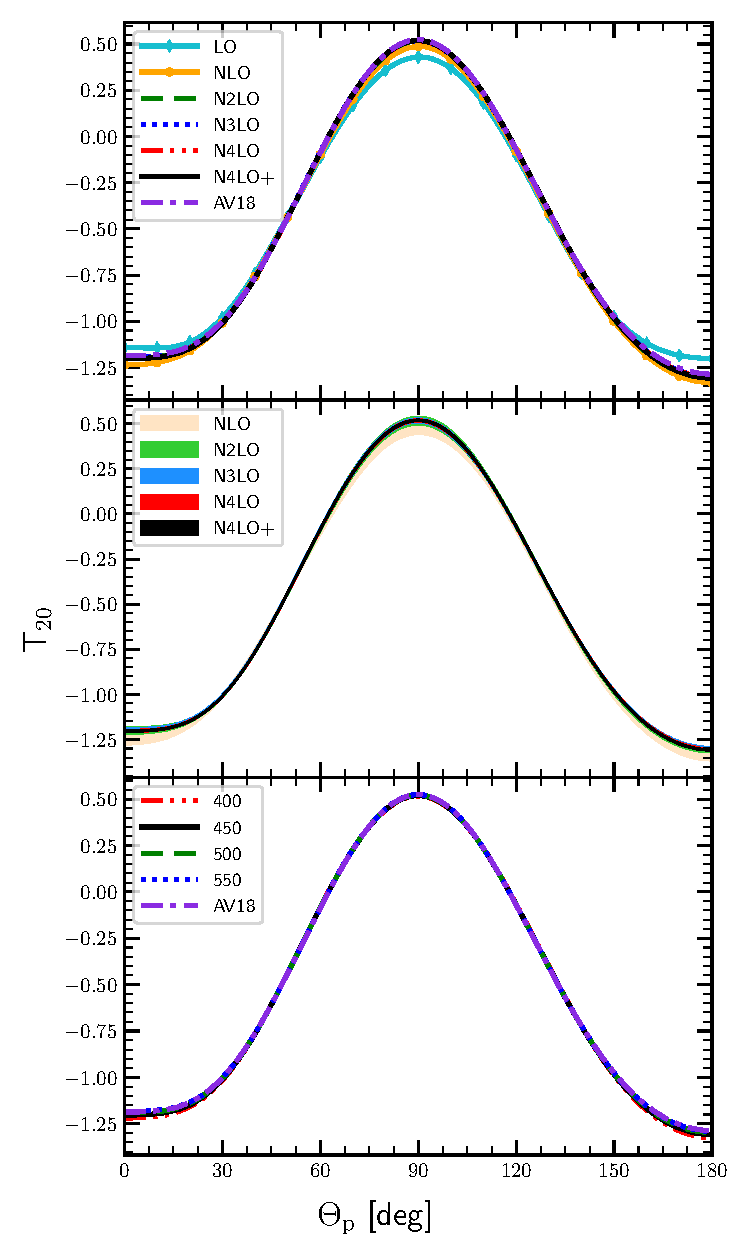
\includegraphics[width=\textwidth]{Figures_python/T20D2_100mev.pdf}
            \caption{T$_{20}$}
            \label{T20_100_vert}
        \end{subfigure}
        \begin{subfigure}[b]{0.46\textwidth}
            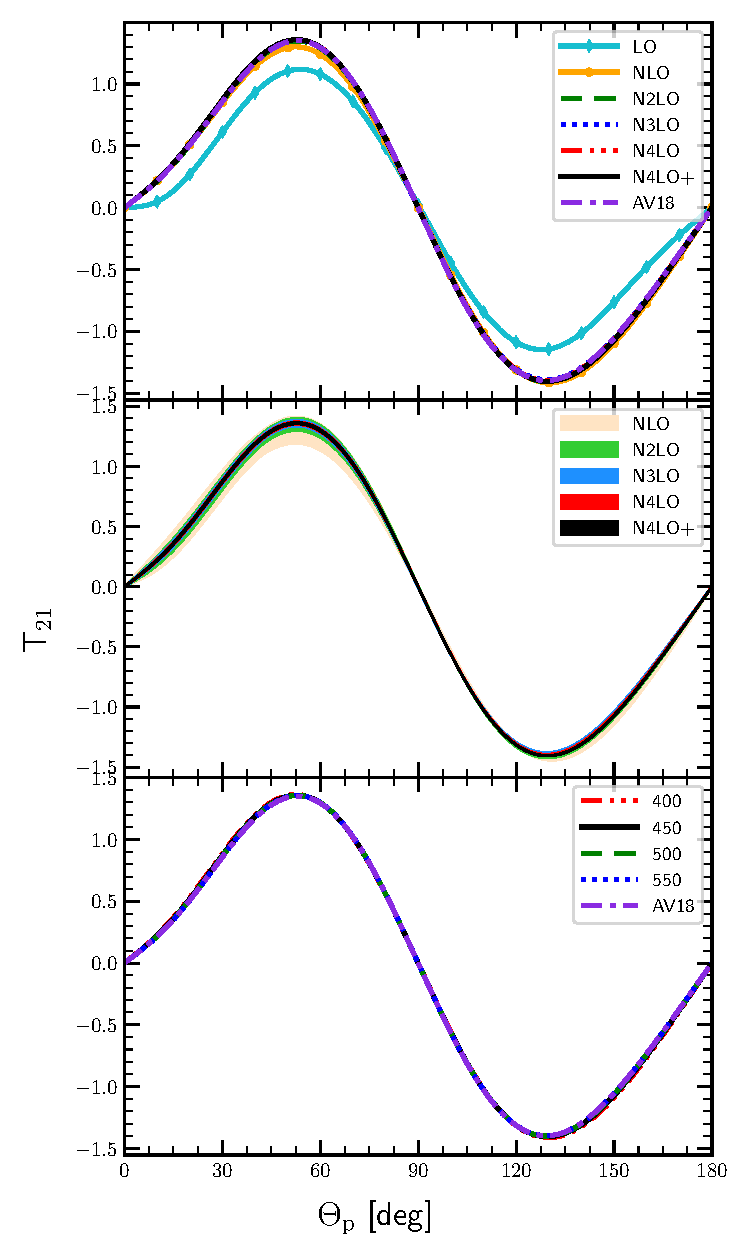
\includegraphics[width=\textwidth]{Figures_python/T21D2_100mev.pdf}
            \caption{T$_{21}$}
            \label{T21_100_vert}
        \end{subfigure}
        \caption{Tensor analyzing power T$_{20}$ (subfigure {\bf (a)})
        and T$_{21}$ (subfigure {\bf (b)})
        as a function of the outgoing proton angle in the center of mass frame 
        for the photon's energy 100 MeV.
        Top row presents results obtained using potential
        with different chiral orders (from LO to N$^4$LO+) with cutoff parameter $\Lambda=450$~MeV.
        The middle row shows truncation errors for each 
        chiral order starting from NLO and
        bottom row presents a cutoff dependency (chiral potential N$^4$LO+).
        For the sake of comparison, predictions obtained with AV18 potential are on figures as well.}
        \label{T20_T21_100}
    \end{figure}

    % \begin{figure}[h]
    %     \begin{center}
    %     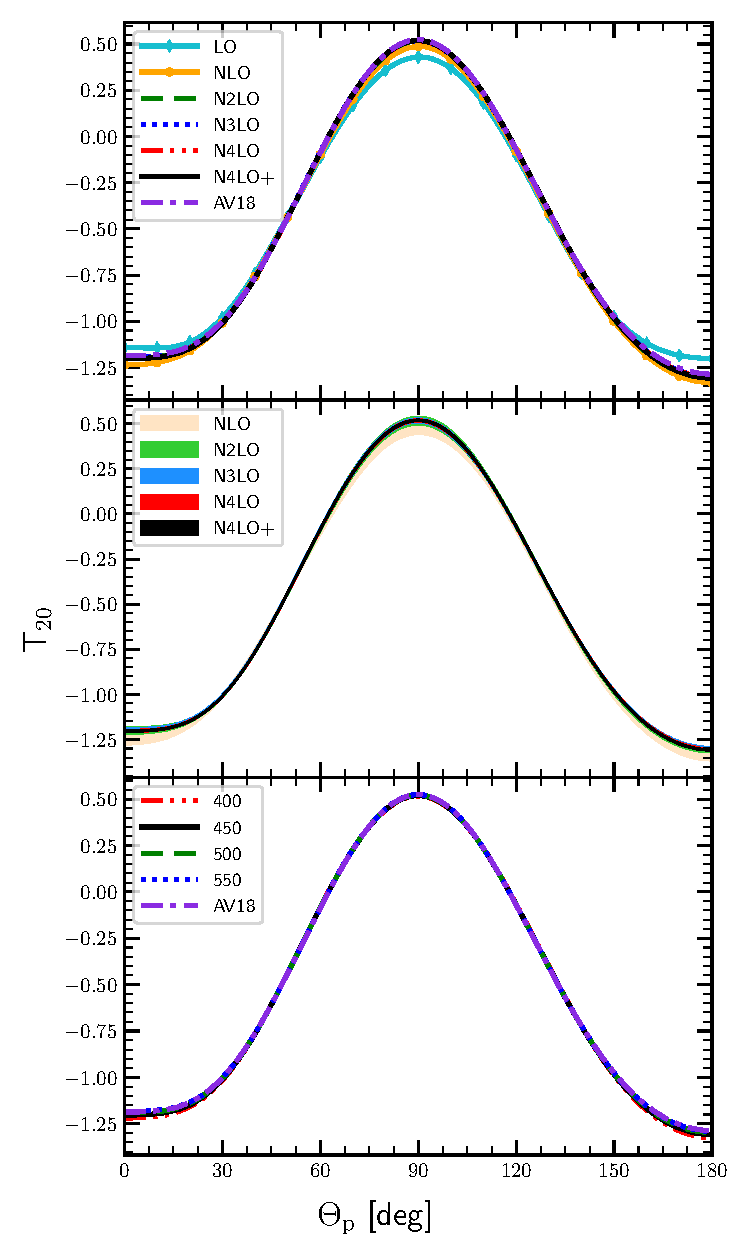
\includegraphics[width=0.6\textwidth]{Figures_python/T20D2_100mev.pdf}
    %     \end{center}
    %     \caption{Tensor analyzing power T$_{20}$ 
    %     as a function of the outgoing proton angle in the center of mass frame 
    %     for the photon's energy 100 MeV.
    %     Top figure presents results obtained using potential
    %     with different chiral orders (from LO to N$^4$LO+) with cutoff parameter $\Lambda=450$~MeV.
    %     The middle pane shows truncation errors for each 
    %     chiral order starting from NLO and
    %     bottom figure presents a cutoff dependency (chiral potential N$^4$LO+).
    %     For the sake of comparison, predictions obtained with AV18 potential are on  figures as well.}
    %     \label{T20_100_vert}
    % \end{figure}

    % \begin{figure}[h]
    %     \begin{center}
    %     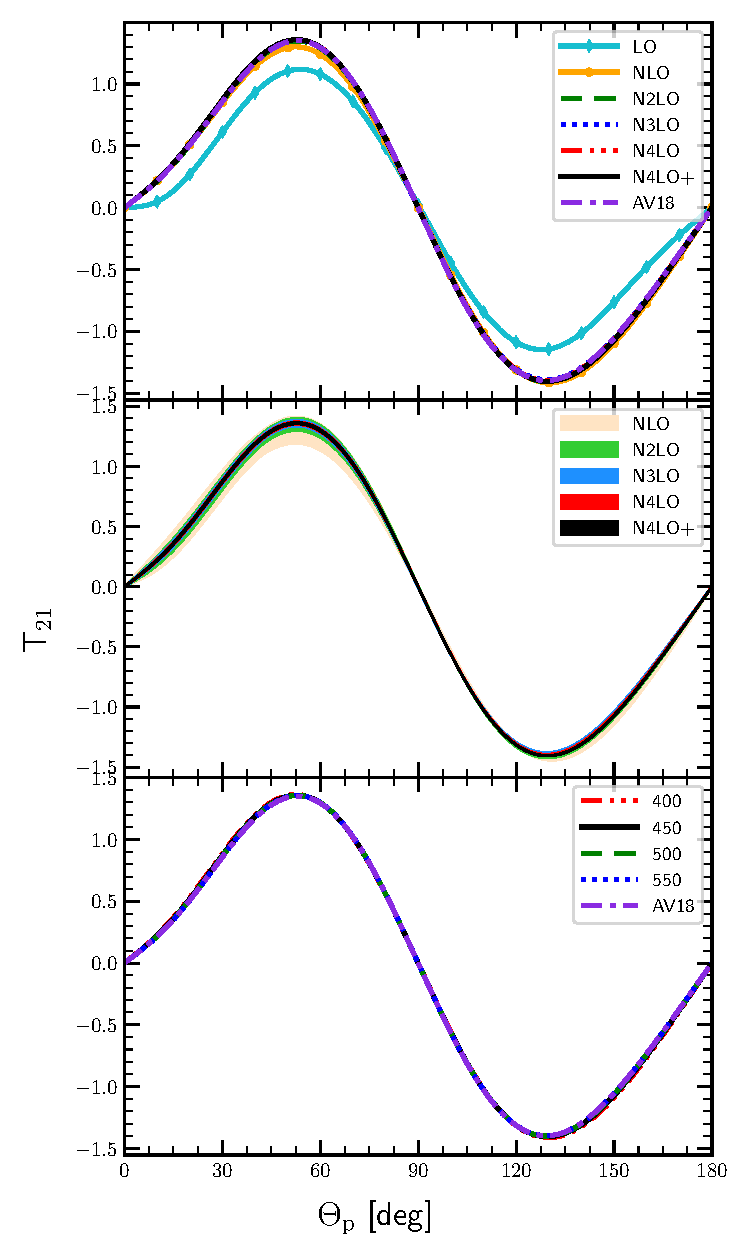
\includegraphics[width=0.7\textwidth]{Figures_python/T21D2_100mev.pdf}
    %     \end{center}
    %     \caption{The same as on \ref{T20_100_vert} but for the 
    %     tensor analyzing power component T$_{21}$}
    %     \label{T21_100_vert}
    % \end{figure}
      
    \begin{figure}[htb]
        \centering
        \begin{subfigure}[b]{0.46\textwidth}
            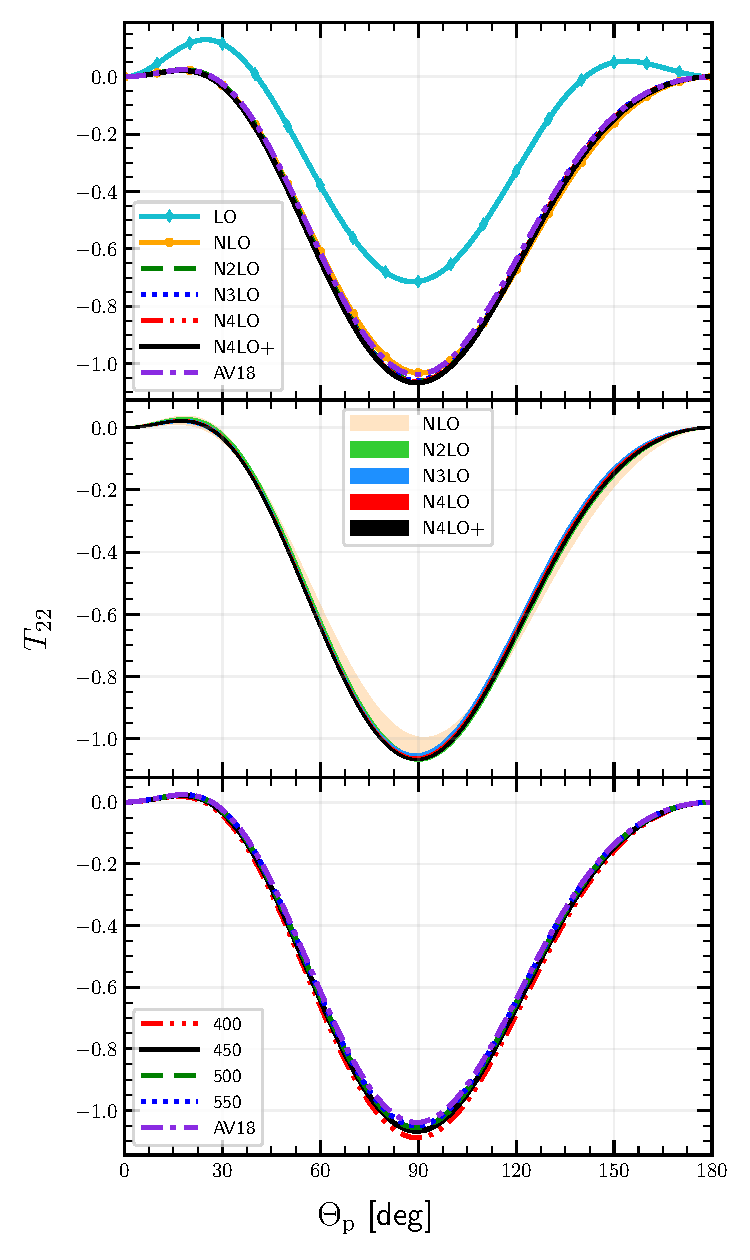
\includegraphics[width=\textwidth]{Figures_python/T22D2_100mev.pdf}
            \caption{T$_{22}$}
            \label{T22_100_vert}
        \end{subfigure}
        \begin{subfigure}[b]{0.46\textwidth}
            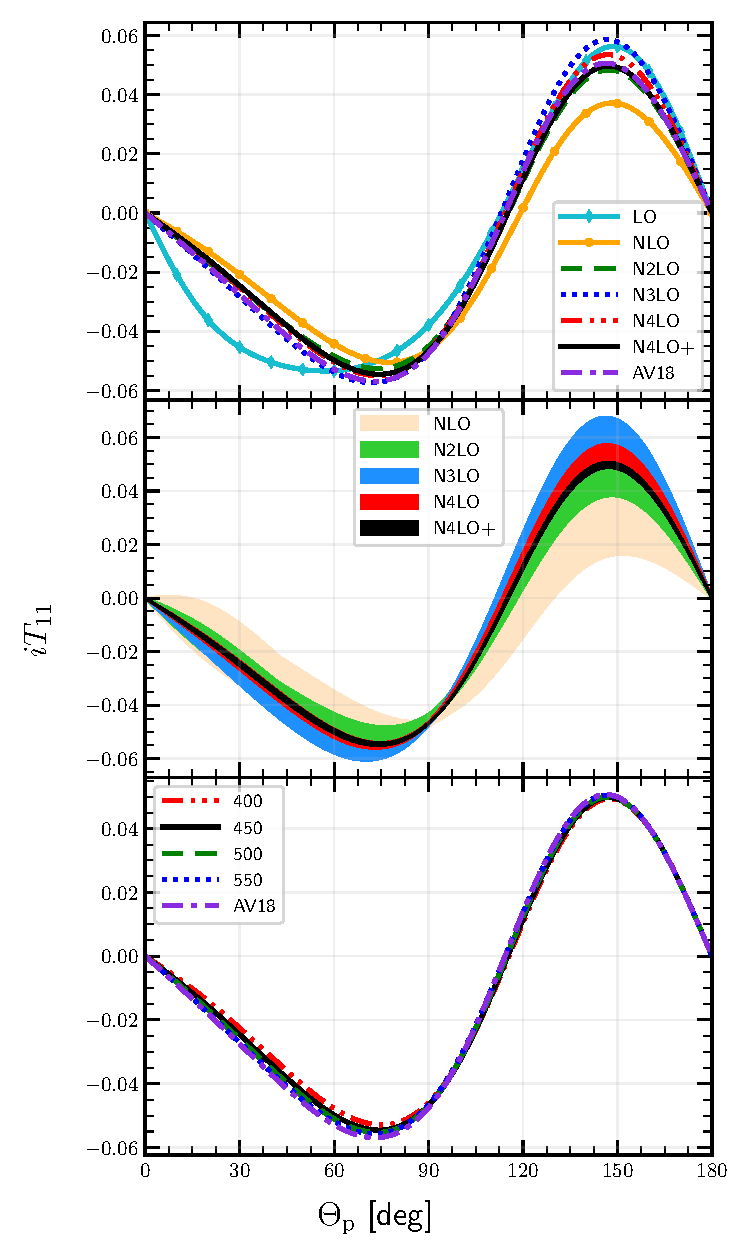
\includegraphics[width=\textwidth]{Figures_python/T11D2_100mev.pdf}
            \caption{iT$_{11}$}
            \label{T11_100_vert}
        \end{subfigure}
        \caption{The same as on \ref{T20_T21_100} but for polarisation observables
        T$_{22}$ (subfigure {\bf (a)}) and iT$_{11}$ (subfigure {\bf (b)}).}
    \end{figure}

    % \begin{figure}[h]
    %     \begin{center}
    %     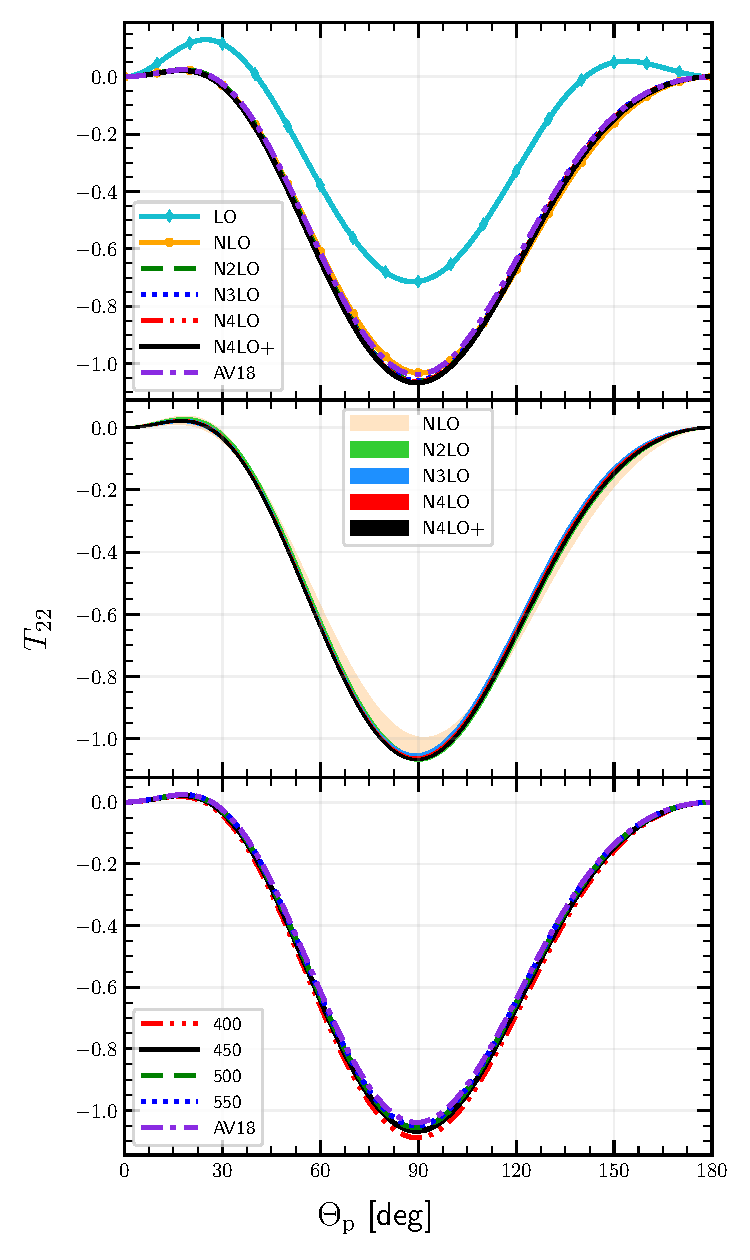
\includegraphics[width=0.7\textwidth]{Figures_python/T22D2_100mev.pdf}
    %     \end{center}
    %     \caption{The same as on \ref{T20_100_vert} but for the 
    %     tensor analyzing power component T$_{22}$}
    %     \label{T22_100_vert}
    % \end{figure}

    
    On the next figures, I show the predictions in a similar way as it was done
    in \cite{rachek2007} in order to compare my predictions with the experimental
    data. On the Figures \ref{tensor_angular_25-45} - \ref{tensor_angular_230-330}
    I show an angular dependance of the $T_{2i}$ ($i=0,1,2$) for a specific energy bands.
    Solid blue line shows an average value of the observable in the specified energy range
    obtained at N$^4$LO+ with $\Lambda=450$~MeV, while the pink dashed line is a prediction
    obtained with a same setup but without using a contributions from Siegert approach
    (single nucleon current only). Bands for each of prediction specify the spread of
    predictions in regarded energy band.
    
    One can see that the data description is better for the predictions with Siegert contributions 
    and SN current is not able to describe experiment properly. With increasing energy 
    (more than 100 MeV),
    the difference between predicted values and experimental data becomes larger
    (especially for $T_{22}$), but the model I use is not meant to be used for high energies 
    and figures are presented out of the curiosity. 
    




    \begin{figure}[h]
        \begin{center}
        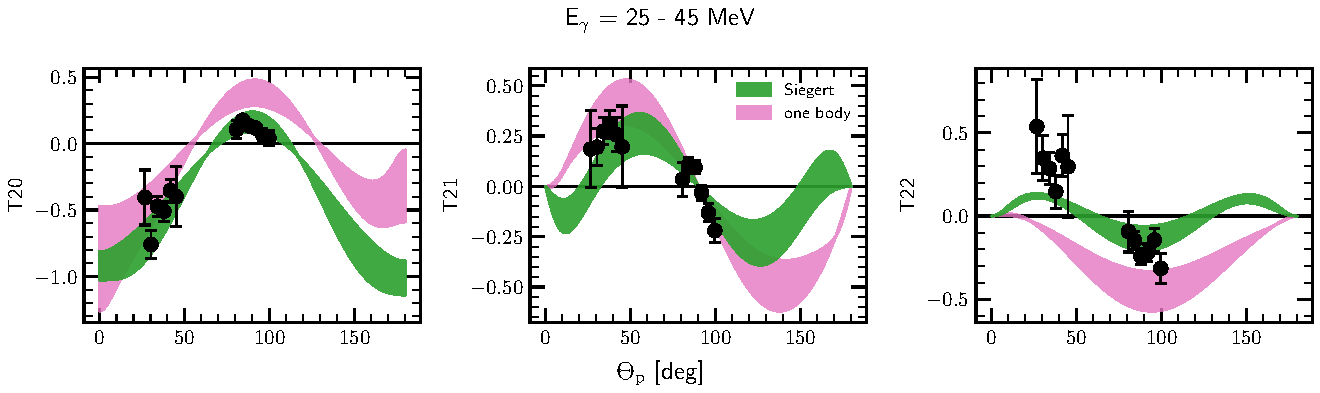
\includegraphics[width=1\textwidth]{Figures_python/Tensor_analyzing_power_angular_E25-45.pdf}
        \end{center}
        \caption{Tensor analyzing powers T$_{20}$, T$_{21}$ and T$_{22}$ as a functions of the
        outgoing proton angle $\theta_p$ (in the center of mass frame).
        Solid blue line is a mean value of my predictions obtained with a
        SMS potential at N$^4$LO+ chiral order and with $\Lambda$~=~450~MeV
        at energy values from 25 to 45 MeV and
        where SN current was used together with Siegert approach. 
        Pink dashed line is similar prediction but with SN only. 
        The corresponding bands show the deviation of predictions in the regarded
        energy region.
        % Filled bands show maximal spread of my predictions obtained with a 
        % SMS potential at N$^4$LO+ chiral order and with $\Lambda$~=~450~MeV
        % for the energy span from 25 to 45 MeV. Blue bands correspond to the
        % case where SN current was used together with Siegert approach and 
        % pink bands - to the SN currentonly. 
        Filled circles are experimental data
        from \cite{rachek2007} for the analogous energy span.}
        \label{tensor_angular_25-45}
    \end{figure}

    \begin{figure}[h]
        \begin{center}
        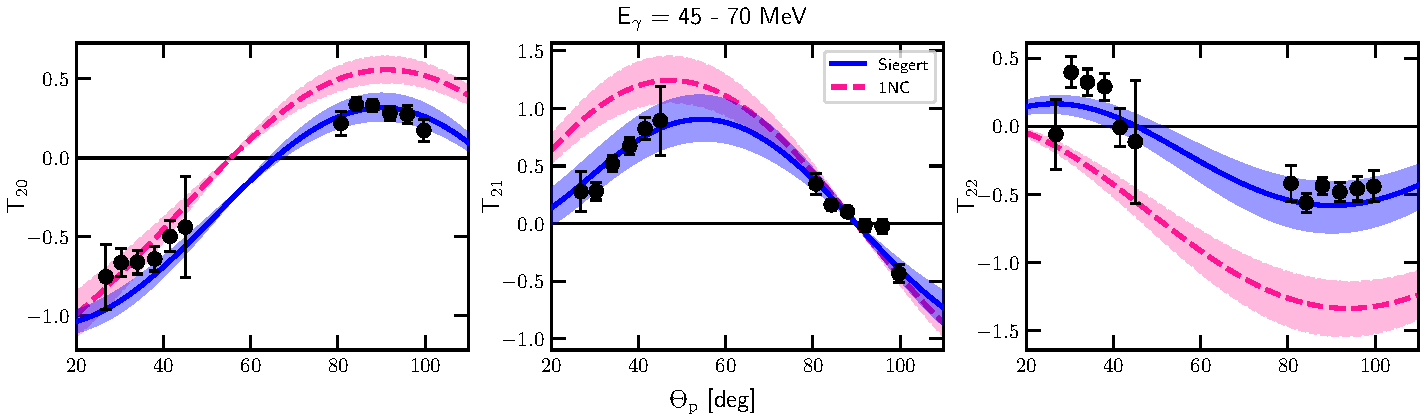
\includegraphics[width=0.95\textwidth]{Figures_python/Tensor_analyzing_power_angular_E45-70.pdf}
        \end{center}
        \caption{The same as on the Fig.~\ref*{tensor_angular_25-45} but for energy bin 45~-~70~MeV}
        \label{tensor_angular_45-70}
    \end{figure}

    \begin{figure}[h]
        \begin{center}
        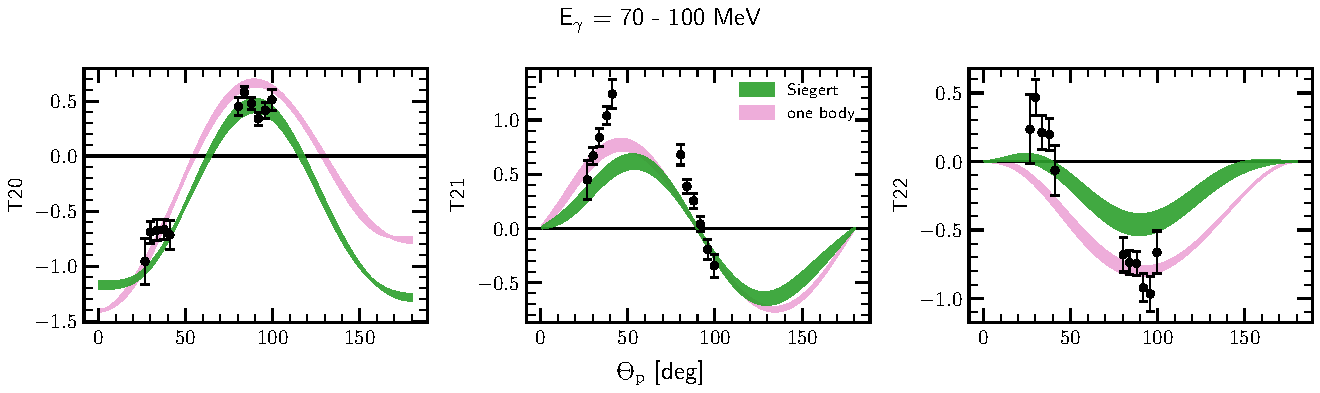
\includegraphics[width=0.95\textwidth]{Figures_python/Tensor_analyzing_power_angular_E70-100.pdf}
        \end{center}
        \caption{The same as on the Fig.~\ref*{tensor_angular_25-45} but for energy bin 70~-~100~MeV}
        \label{tensor_angular_70-100}
    \end{figure}        

    \begin{figure}[h]
        \begin{center}
        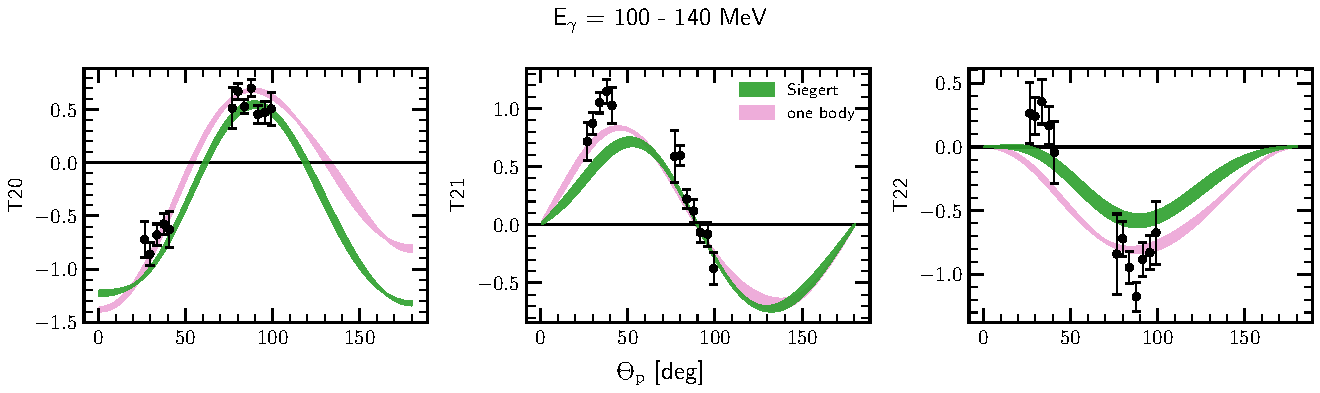
\includegraphics[width=0.95\textwidth]{Figures_python/Tensor_analyzing_power_angular_E100-140.pdf}
        \end{center}
        \caption{The same as on the Fig.~\ref*{tensor_angular_25-45} but for energy bin 100~-~140~MeV}
        \label{tensor_angular_100-140}
    \end{figure}
        
        

    \begin{figure}[h]
        \begin{center}
        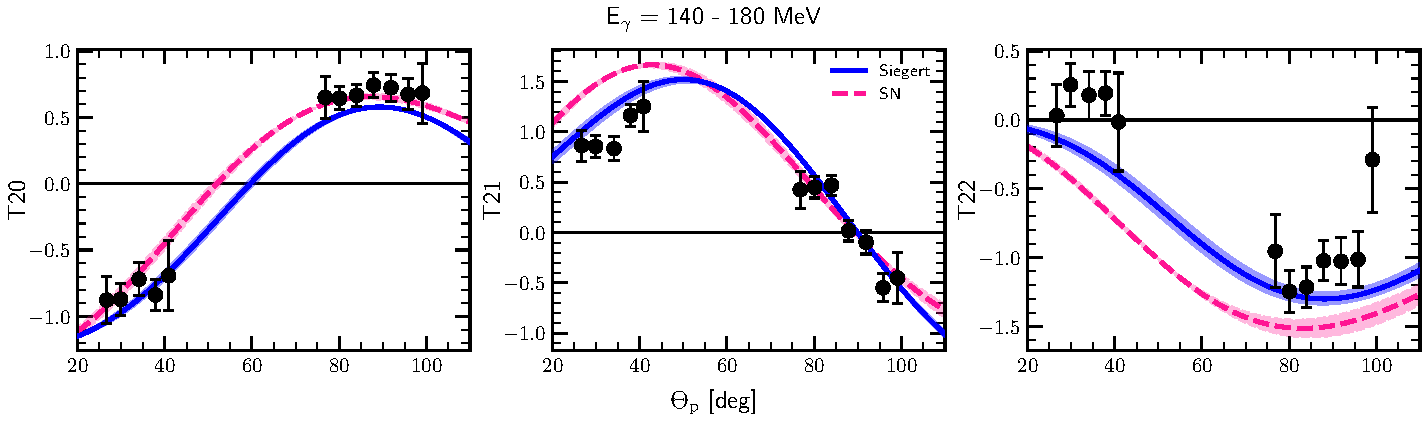
\includegraphics[width=0.95\textwidth]{Figures_python/Tensor_analyzing_power_angular_E140-180.pdf}
        \end{center}
        \caption{The same as on the Fig.~\ref*{tensor_angular_25-45} but for energy bin 140~-~180~MeV}
        \label{tensor_angular_140-180}
    \end{figure}
        

    \begin{figure}[h]
        \begin{center}
        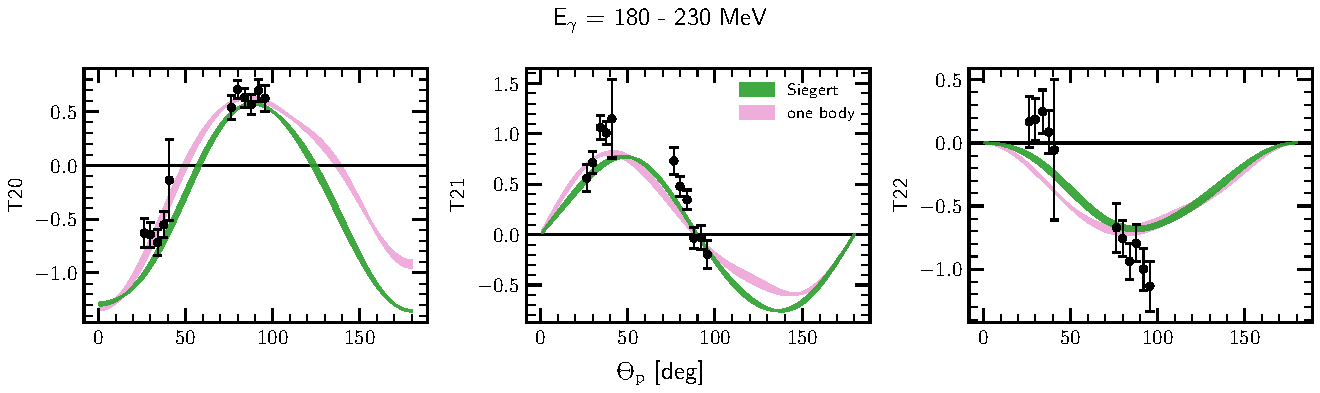
\includegraphics[width=0.95\textwidth]{Figures_python/Tensor_analyzing_power_angular_E180-230.pdf}
        \end{center}
        \caption{The same as on the Fig.~\ref*{tensor_angular_25-45} but for energy bin 180~-~230~MeV}
        \label{tensor_angular_180-230}
    \end{figure}

    \begin{figure}[h]
        \begin{center}
        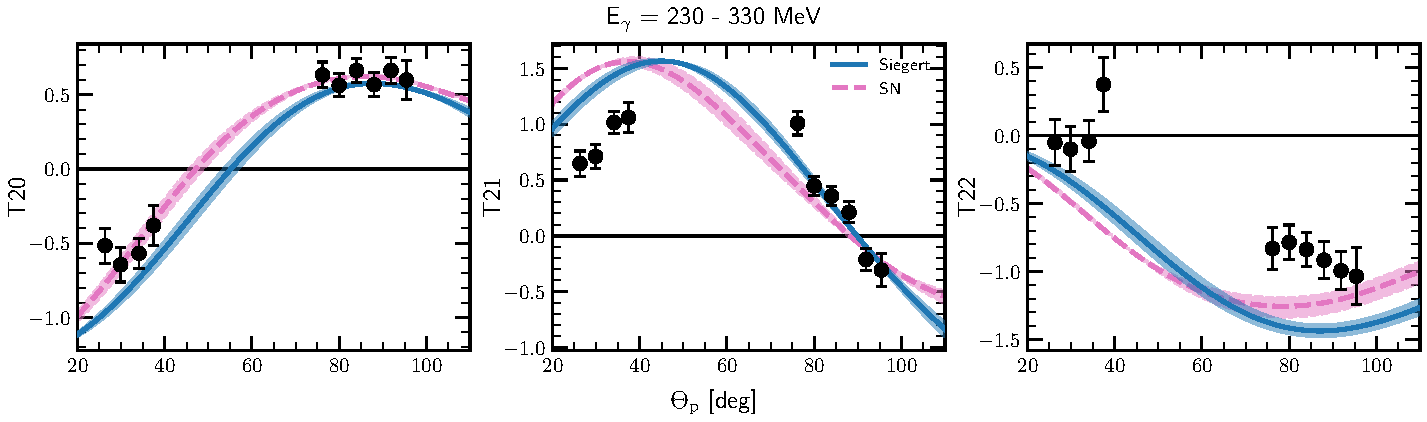
\includegraphics[width=0.95\textwidth]{Figures_python/Tensor_analyzing_power_angular_E230-330.pdf}
        \end{center}
        \caption{The same as on the Fig.~\ref*{tensor_angular_25-45} but for energy bin 230~-~330~MeV}
        \label{tensor_angular_230-330}
    \end{figure}
        


    On the Figure \ref{T20_vs_en} the energy dependance of $T_{20}$ and $T_{22}$
    (integrated over all angles)
    is presented for the energy range 0-400~MeV. I also demonstrate the experimental data from
    \cite{rachek2007} and \cite{mishev1993} as well as theoretical calculations from \cite{Schmitt1989}
    on the figure. For $T_{20}$ the model is able to describe experimental data well even for
    high energies. On the other hand, $T_{22}$ is not so well described: for the low 
    energies the prediction curve is somehow within uncertainties of experimental data,
    but further the difference with the data becomes larger. Also it is not 
    reflect the qualitative nature of the data as we can see that after around 150~MeV
    data points start ascending which is not represented in my predictions.
    Theoretical predictions from \cite{Schmitt1989} (brown dashed curve) are also not able
    to describe data quantitatively for $T_{22}$, but the growth is presented there. 

    Similar situation is on the Figures \ref{tensor_energy_24-48} and \ref{tensor_energy_70-102}
    where I show an energy dependance of Deuteron analyzing power components for 
    specific angular ranges (following the data from \cite{rachek2007}).
    Predictions for $T_{20}$ are able to reflect the experimental results,
    while for $T_{21}$ and $T_{22}$ predictions are reasonable (quantitative-wise) 
    only for lower energies and difference with data becomes larger
    when energy increases. Predictions for $T_{22}$ once more 
    confirm an insufficiency of SN and an importance of
    2-nucleon current contributions. 
    

    \begin{figure}[h]
        \begin{center}
        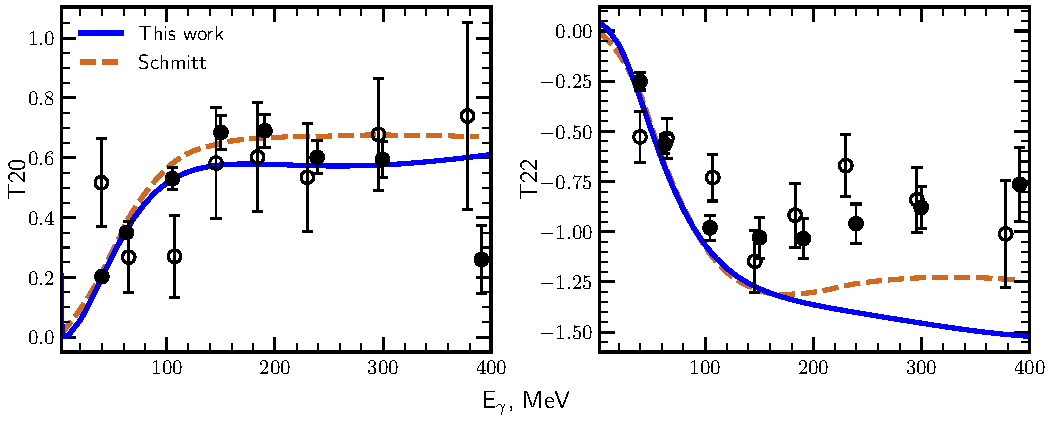
\includegraphics[width=0.9\textwidth]{Figures_python/T20_T22_vs_en.pdf}
        \end{center}
        \caption{Tensor analyzing powers T$_{20}$ and T$_{22}$ as a functions of the photon energy E$_\gamma$
        with fixed outgoing proton angle $\theta_p = 88^{\circ}$ (in the center of mass frame).
        My predictions (blue solid line) are obtained with SMS potential at chiral order N$^4$LO+
        and with cutoff parameter $\Lambda$~=~450~MeV.
        Dashed brown line presents calculations from \cite{Schmitt1989}.
        Experimental data is taken from \cite{rachek2007} (filled circles)
        and \cite{mishev1993} (empty circles).}
        \label{T20_vs_en}
    \end{figure}

    \begin{figure}[h]
        \begin{center}
        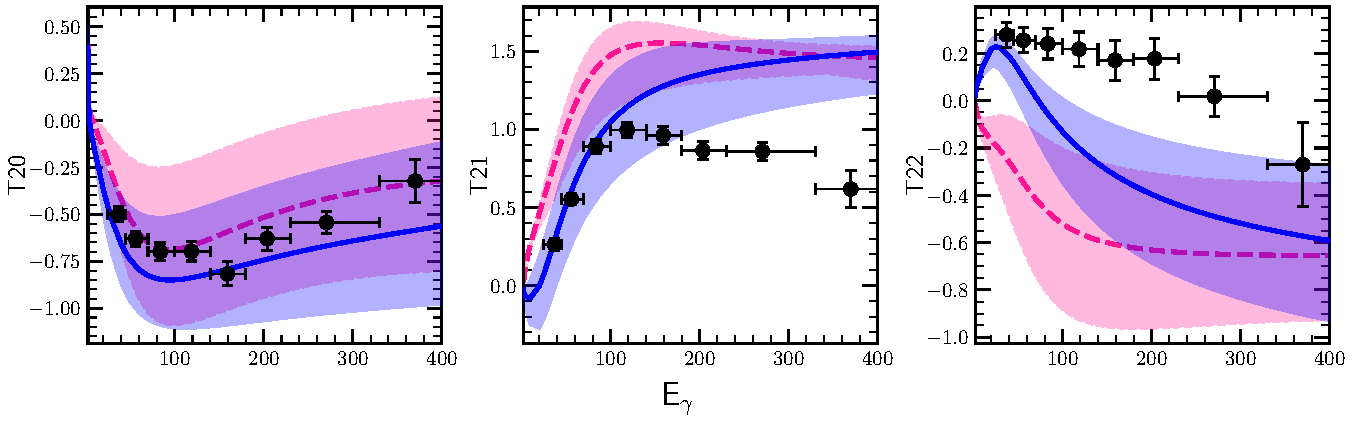
\includegraphics[width=0.95\textwidth]{Figures_python/TensorPower_Th24-48.pdf}
        \end{center}
        \caption{Tensor analyzing powers T$_{20}$, T$_{21}$ and T$_{22}$ as a functions of the
        photon's energy within the outgoing proton's angle range $24^{\circ} - 48^{\circ}$
        (in the center of mass frame).
        Solid blue line is a mean value of my predictions obtained with
        SMS potential at N$^4$LO+ chiral order and with $\Lambda$~=~450~MeV
        at energy values from 25 to 45 MeV within
        a given angles range and
        where SN current was used together with Siegert approach. 
        Pink dashed line is similar prediction but with SN only. 
        The corresponding bands show the deviation of predictions in the regarded
        energy region.
        Filled circles are experimental data
        from \cite{rachek2007} for the analogous energy span.}
        \label{tensor_energy_24-48}
    \end{figure}

    \begin{figure}[h]
        \begin{center}
        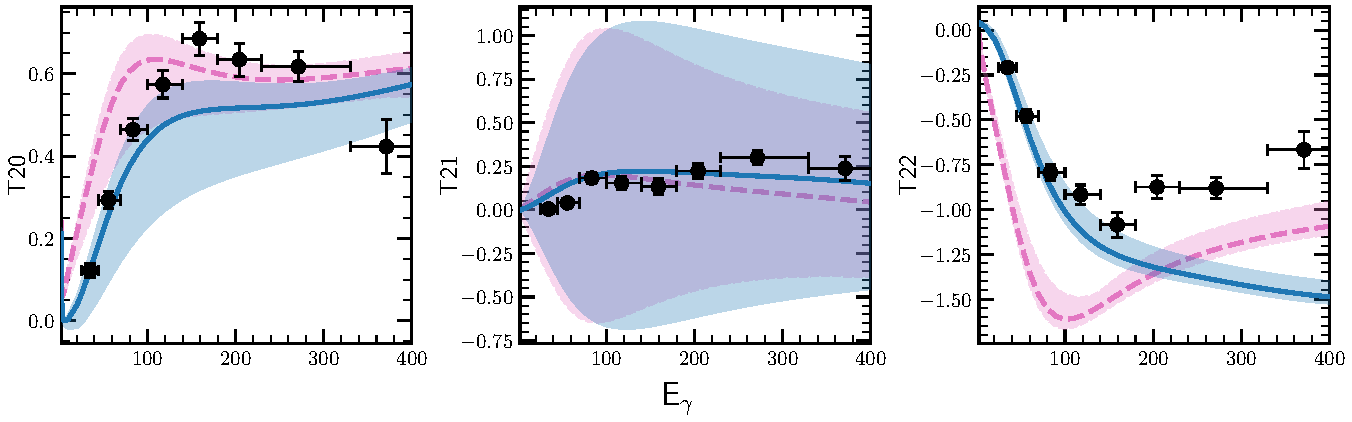
\includegraphics[width=0.95\textwidth]{Figures_python/TensorPower_Th70-102.pdf}
        \end{center}
        \caption{The same as on the Fig.~\ref*{tensor_energy_24-48} but
        for the angles' range $70^{\circ} - 102^{\circ}$.}
        \label{tensor_energy_70-102}
    \end{figure}
    
    
    % \begin{figure}[h]
    %     \begin{center}
    %     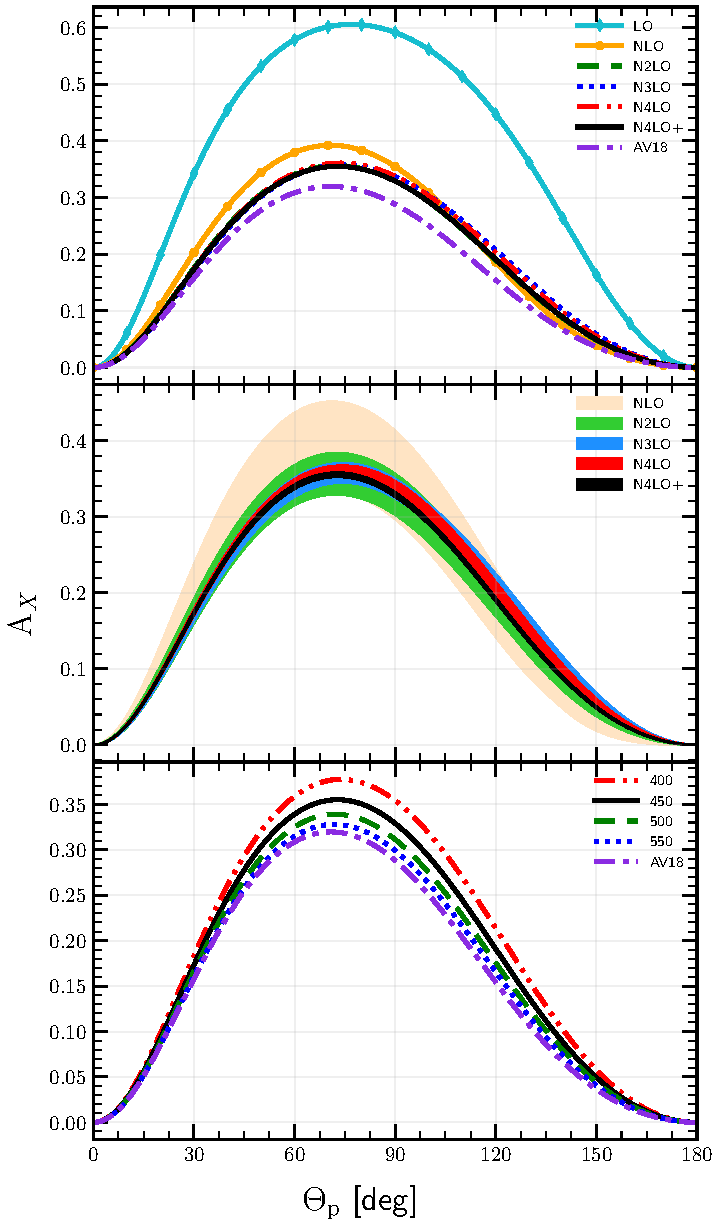
\includegraphics[width=0.6\textwidth]{Figures_python/AX2_100mev.pdf}
    %     \end{center}
    %     \caption{The photon asymmetry $\Sigma_\gamma$ 
    %     as a function of the outgoing proton angle in the center of mass frame 
    %     for the photon's energy 100 MeV.
    %     Top figure presents results obtained using potential
    %     with different chiral orders (from LO to N$^4$LO+) with cutoff parameter $\Lambda=450$~MeV.
    %     The middle pane shows truncation errors for each 
    %     chiral order starting from NLO and
    %     bottom figure presents a cutoff dependency (chiral potential N$^4$LO+).
    %     For the sake of comparison, predictions obtained with AV18 potential are on  figures as well.}
    %     \label{AX_100_vert}
    % \end{figure}
    \begin{figure}[h]
        \centering
        \begin{subfigure}[b]{0.46\textwidth}
            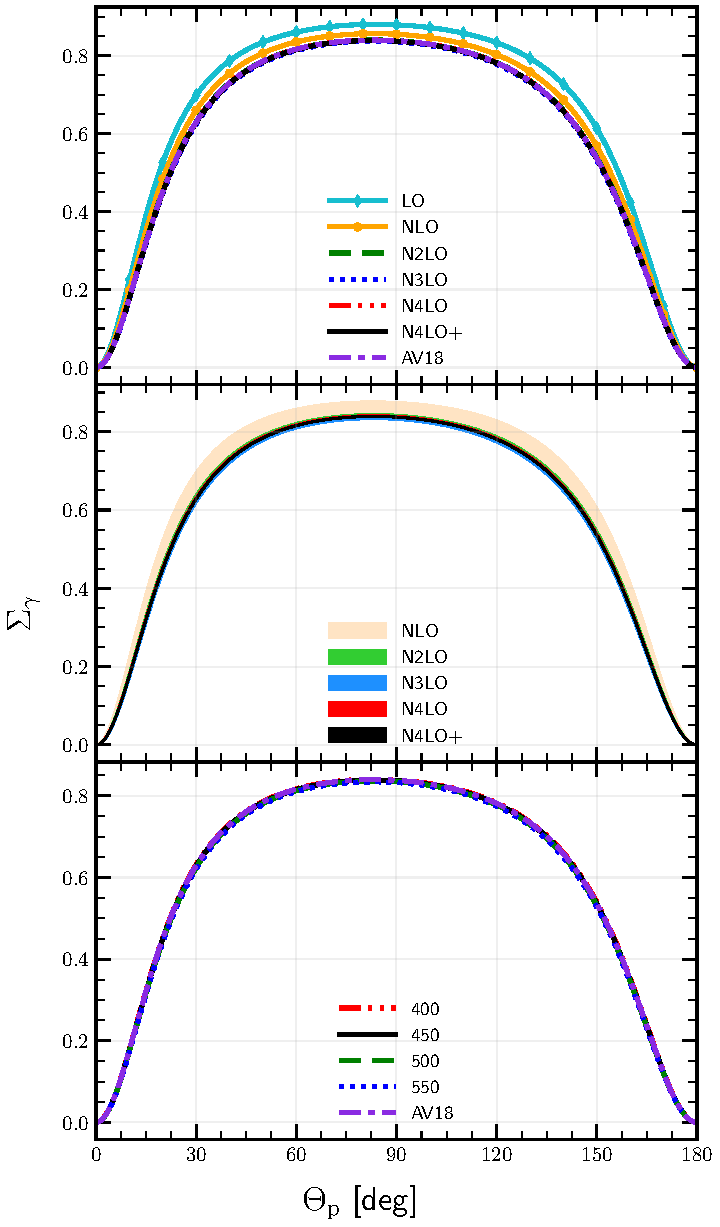
\includegraphics[width=\textwidth]{Figures_python/AX2_30mev.pdf}
            \caption{\small E$_\gamma = 30$~MeV}
            \label{AX_30_vert}
        \end{subfigure}
        \begin{subfigure}[b]{0.46\textwidth}
            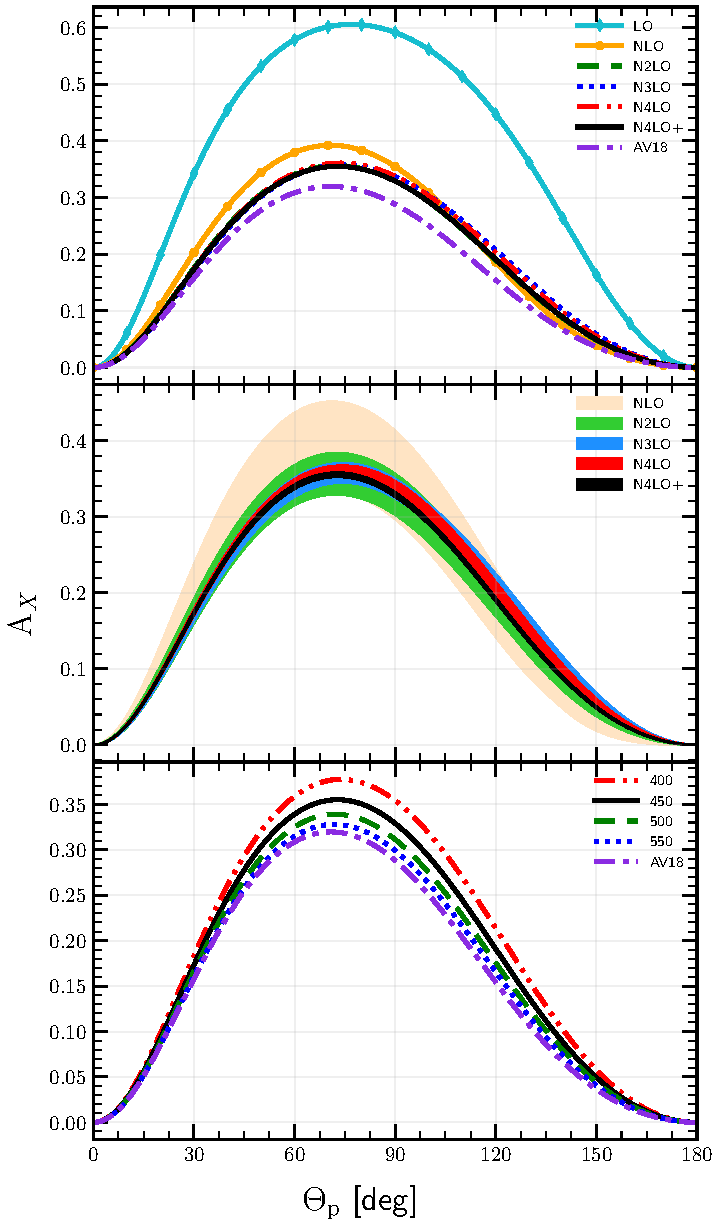
\includegraphics[width=\textwidth]{Figures_python/AX2_100mev.pdf}
            \caption{\small E$_\gamma = 100$~MeV}
            \label{AX_100_vert}
        \end{subfigure}
        \caption{The photon asymmetry $\Sigma_\gamma$ 
        as a function of the outgoing proton angle in the center of mass frame 
        for the photon's energy 100 MeV.
        Top figure presents results obtained using potential
        with different chiral orders (from LO to N$^4$LO+) with cutoff parameter $\Lambda=450$~MeV.
        The middle pane shows truncation errors for each 
        chiral order starting from NLO and
        bottom figure presents a cutoff dependency (chiral potential N$^4$LO+).
        For the sake of comparison, predictions obtained with AV18 potential are on  figures as well.}
    \end{figure}
     
    % \begin{figure}[h]
    %     \begin{center}
    %     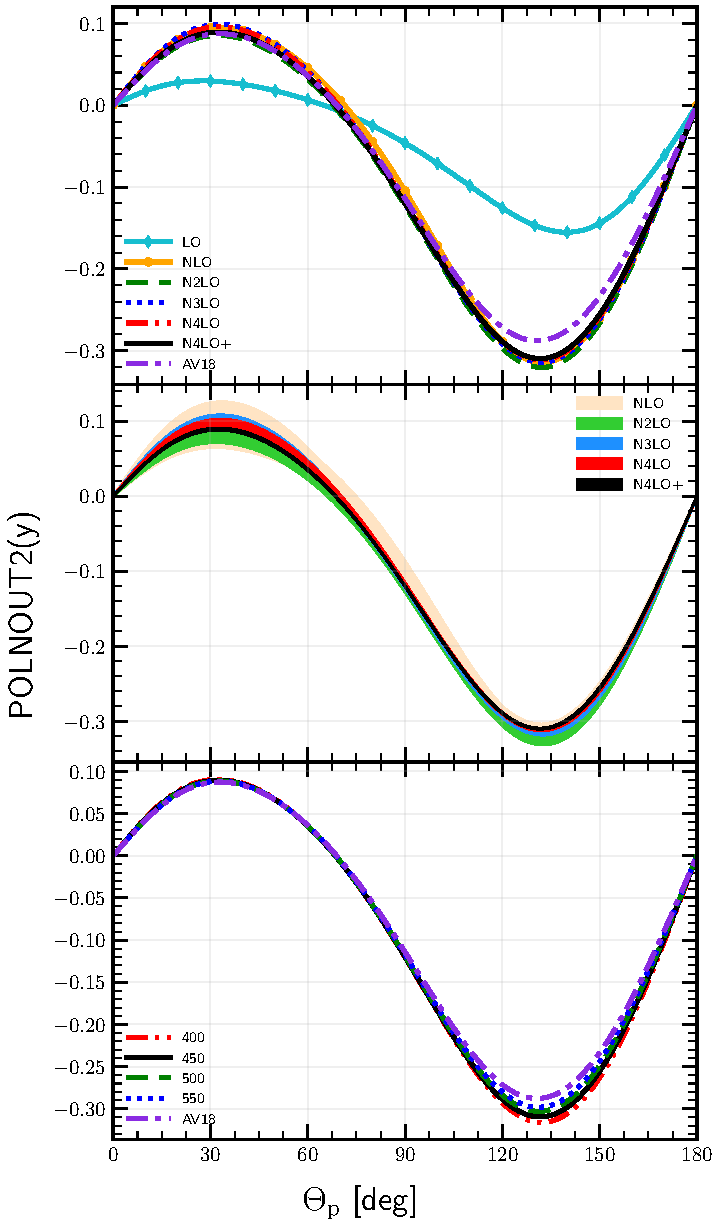
\includegraphics[width=0.6\textwidth]{Figures_python/POLNOUT2(y)_100mev.pdf}
    %     \end{center}
    %     \caption{Proton polarisation $P_y$ 
    %     as a function of the outgoing proton angle in the center of mass frame 
    %     for the photon's energy 100 MeV.
    %     Top figure presents results obtained using potential
    %     with different chiral orders (from LO to N$^4$LO+) with cutoff parameter $\Lambda=450$~MeV.
    %     The middle pane shows truncation errors for each 
    %     chiral order starting from NLO and
    %     bottom figure presents a cutoff dependency (chiral potential N$^4$LO+).
    %     For the sake of comparison, predictions obtained with AV18 potential are on  figures as well.}
    %     \label{PY_100_vert}
    % \end{figure}
    
    \begin{figure}[h]
        \centering
        \begin{subfigure}[b]{0.46\textwidth}
            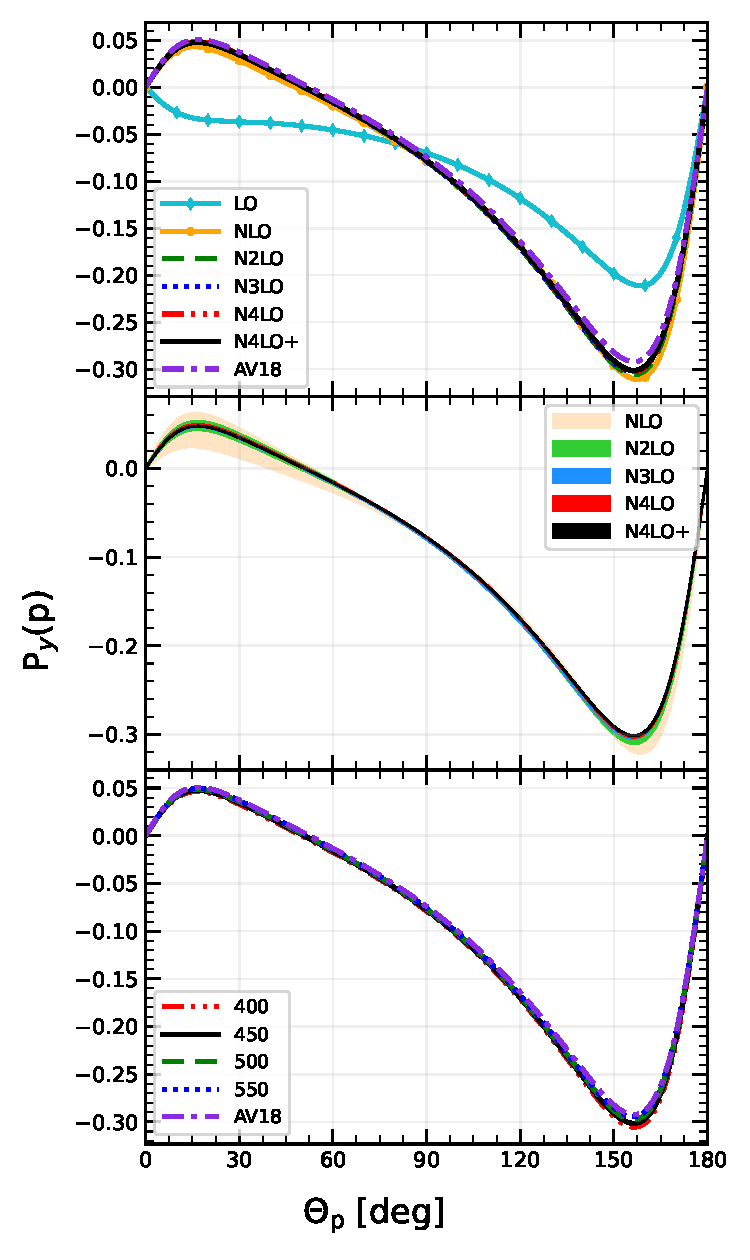
\includegraphics[width=\textwidth]{Figures_python/POLNOUT2(y)_30mev.pdf}
            \caption{\small E$_\gamma = 30$~MeV}
            \label{PY_30_vert}
        \end{subfigure}
        \begin{subfigure}[b]{0.46\textwidth}
            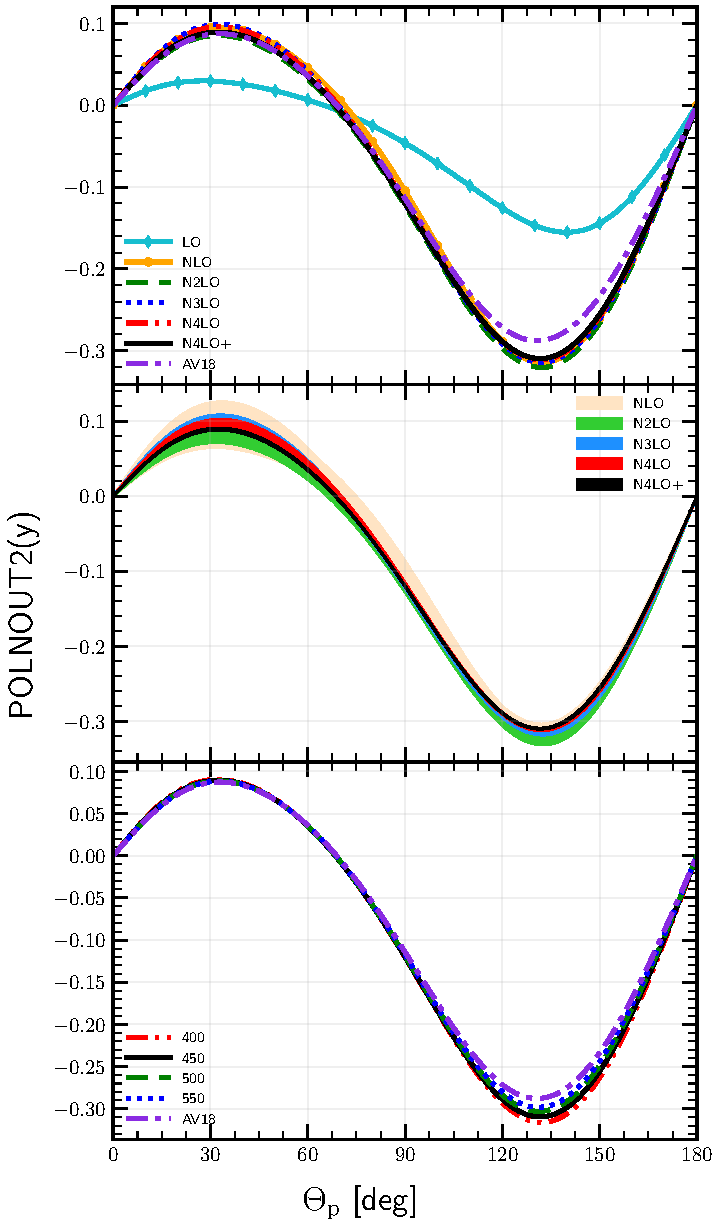
\includegraphics[width=\textwidth]{Figures_python/POLNOUT2(y)_100mev.pdf}
            \caption{\small E$_\gamma = 100$~MeV}
            \label{PY_100_vert}
        \end{subfigure}
        \caption{Proton polarisation $P_y$ 
        as a function of the outgoing proton angle in the center of mass frame 
        for the photon's energy 30 MeV (a) and 100 MeV (b).
        Top figure presents results obtained using potential
        with different chiral orders (from LO to N$^4$LO+) with cutoff parameter $\Lambda=450$~MeV.
        The middle pane shows truncation errors for each 
        chiral order starting from NLO and
        bottom figure presents a cutoff dependency (chiral potential N$^4$LO+).
        For the sake of comparison, predictions obtained with AV18 potential are on  figures as well.}
    \end{figure}

\clearpage

\section{Helium photodisintegration}

\subsection{3N photodisintegration}
    \begin{figure}[h]
        \begin{center}
            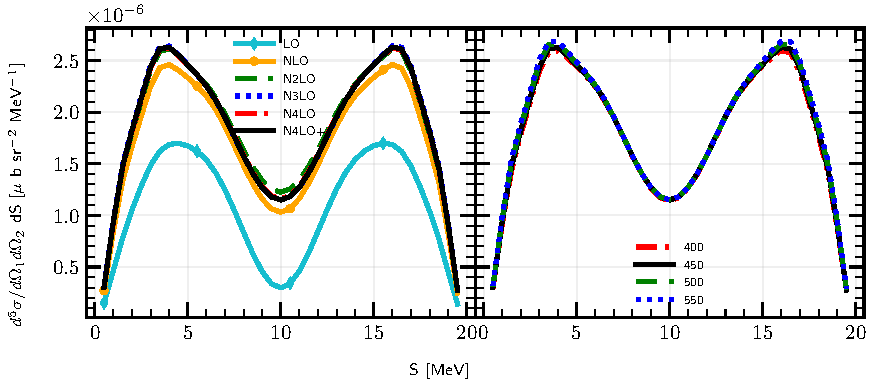
\includegraphics[width=0.9\textwidth]{Figures_HE/CROSS_excl_30mev.pdf}
            \end{center}
            \caption{The five-fold differential cross section for the photon 
            energy E$_\gamma=30$~MeV.
            The left figure presents results obtained using potential
            with different chiral orders (from LO to N$^4$LO+) with cutoff parameter $\Lambda=450$~MeV.
            The right figure presents a cutoff dependency (chiral potential N$^4$LO+).}
            \label{CROSS_HE_EXCL_30}
        \end{figure}

        % \begin{figure}[h]
        %     \begin{center}
        %     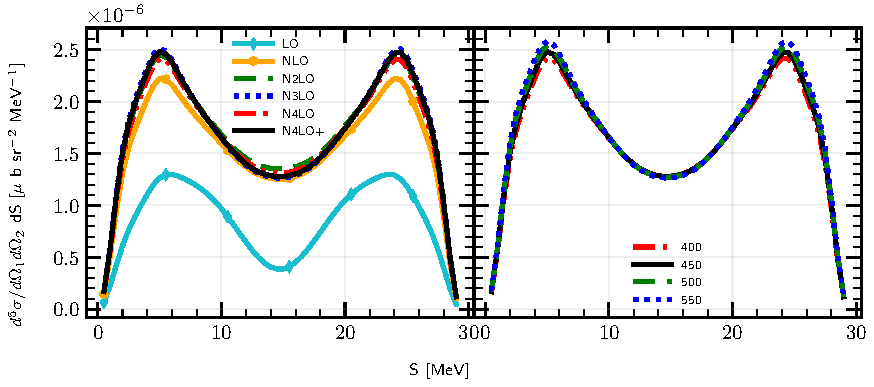
\includegraphics[width=0.9\textwidth]{Figures_HE/CROSS_excl_40mev.pdf}
        %     \end{center}
        %     \caption{The same as on Fig.~\ref{CROSS_HE_EXCL_30} but 
        %     for the photon energy E$_\gamma=40$~MeV}
        %     \label{CROSS_HE_EXCL_40}
        % \end{figure}

        \begin{figure}[h]
            \begin{center}
            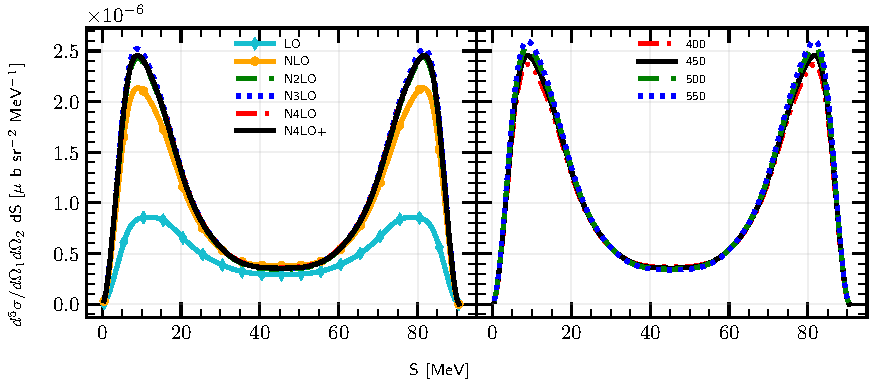
\includegraphics[width=0.9\textwidth]{Figures_HE/CROSS_excl_100mev.pdf}
            \end{center}
            \caption{The same as on Fig.~\ref{CROSS_HE_EXCL_30} but 
            for the photon energy E$_\gamma=100$~MeV}
            \label{CROSS_HE_EXCL_100}
        \end{figure}

        % \begin{figure}[h]
        %     \begin{center}
        %     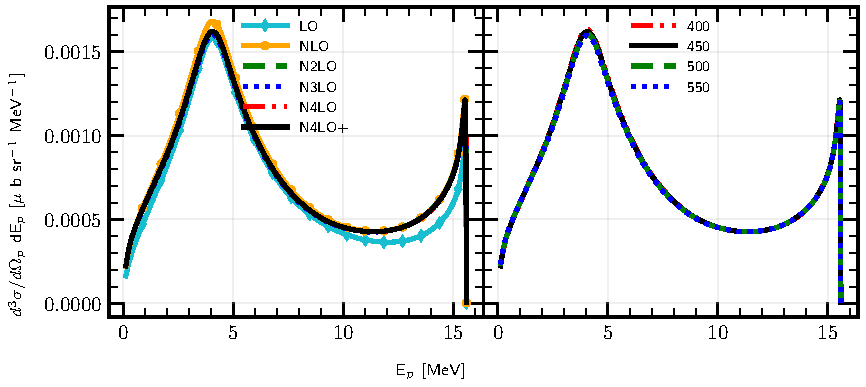
\includegraphics[width=0.9\textwidth]{Figures_HE/CROSS_incl_30mev_60deg.pdf}
        %     \end{center}
        %     \caption{Inclusive cross section... E$_\gamma=30$~MeV, $\theta=60^\circ$ }
        %     \label{CROSS_HE_INCL_30_60deg}
        % \end{figure}

        % \begin{figure}[h]
        %     \begin{center}
        %     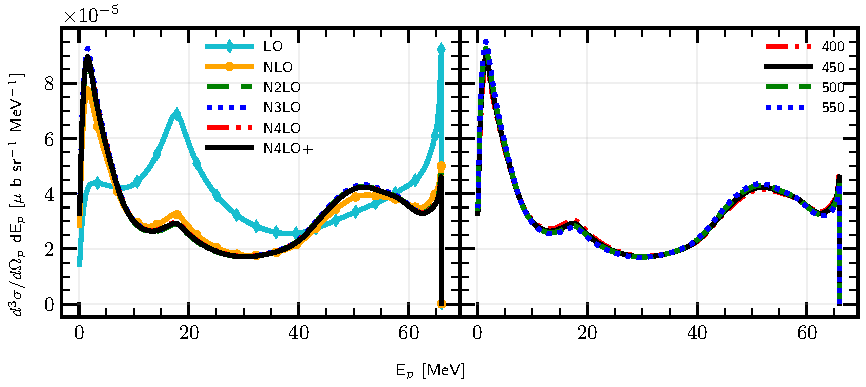
\includegraphics[width=0.9\textwidth]{Figures_HE/CROSS_incl_100mev_60deg.pdf}
        %     \end{center}
        %     \caption{Inclusive cross section...  E$_\gamma=100$~MeV, $\theta=60^\circ$}
        %     \label{CROSS_HE_INCL_100_60deg}
        % \end{figure}

        \begin{figure}[h]
            \centering
            \begin{subfigure}[b]{0.7\textwidth}
                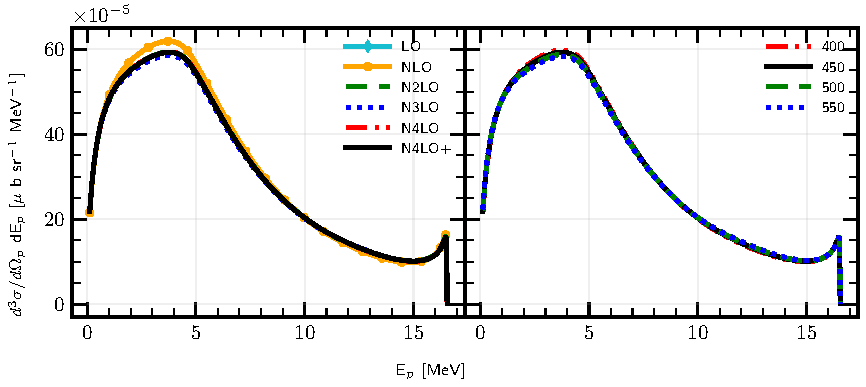
\includegraphics[width=\textwidth]{Figures_HE/CROSS_incl_30mev_10deg.pdf}
                \caption{$\theta_1 = 10^\circ$}
                \label{Diff_cross_truncation}
            \end{subfigure}
            \begin{subfigure}[b]{0.7\textwidth}
                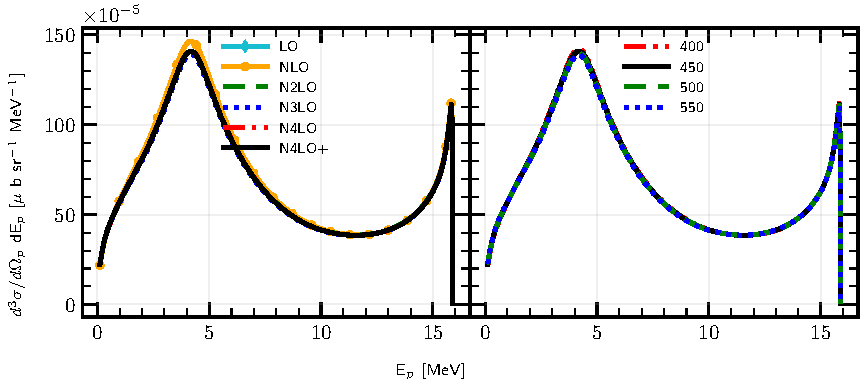
\includegraphics[width=\textwidth]{Figures_HE/CROSS_incl_30mev_50deg.pdf}
                \caption{$\theta_1 = 50^\circ$}
                \label{Diff_cross_cutoff}
            \end{subfigure}
            \begin{subfigure}[b]{0.7\textwidth}
                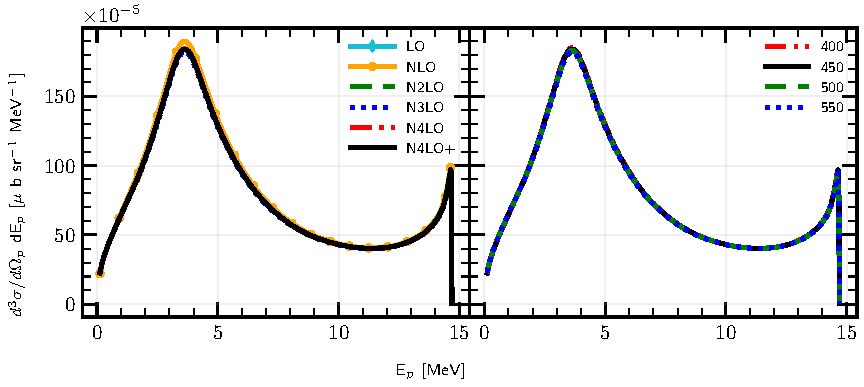
\includegraphics[width=\textwidth]{Figures_HE/CROSS_incl_30mev_90deg.pdf}
                \caption{$\theta_1 = 90^\circ$}
                \label{Diff_cross_cutoff}
            \end{subfigure}
            \begin{subfigure}[b]{0.7\textwidth}
                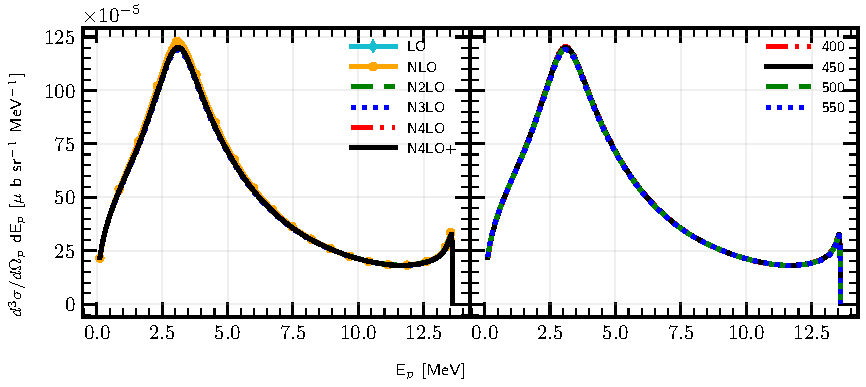
\includegraphics[width=\textwidth]{Figures_HE/CROSS_incl_30mev_130deg.pdf}
                \caption{$\theta_1 = 130^\circ$}
                \label{Diff_cross_cutoff}
            \end{subfigure}
            % \begin{subfigure}[b]{0.7\textwidth}
            %     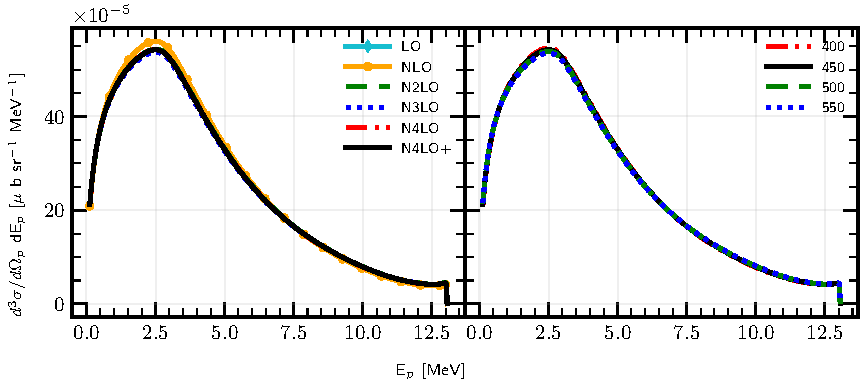
\includegraphics[width=\textwidth]{Figures_HE/CROSS_incl_30mev_170deg.pdf}
            %     \caption{Cutoff dependance}
            %     \label{Diff_cross_cutoff}
            % \end{subfigure}
            
            \caption{Inclusive cross section. E$_\gamma$=30~MeV}
        \end{figure}

        \begin{figure}[h]
            \centering
            \begin{subfigure}[b]{0.7\textwidth}
                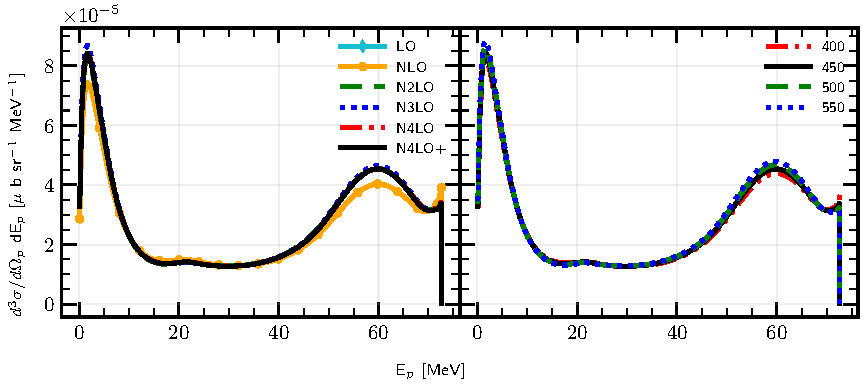
\includegraphics[width=\textwidth]{Figures_HE/CROSS_incl_100mev_10deg.pdf}
                \caption{$\theta_1 = 10^\circ$}
                \label{Diff_cross_truncation}
            \end{subfigure}
            \begin{subfigure}[b]{0.7\textwidth}
                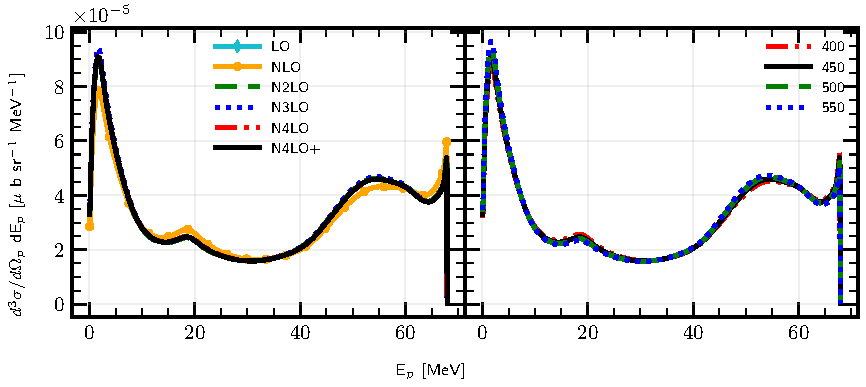
\includegraphics[width=\textwidth]{Figures_HE/CROSS_incl_100mev_50deg.pdf}
                \caption{$\theta_1 = 50^\circ$}
                \label{Diff_cross_cutoff}
            \end{subfigure}
            \begin{subfigure}[b]{0.7\textwidth}
                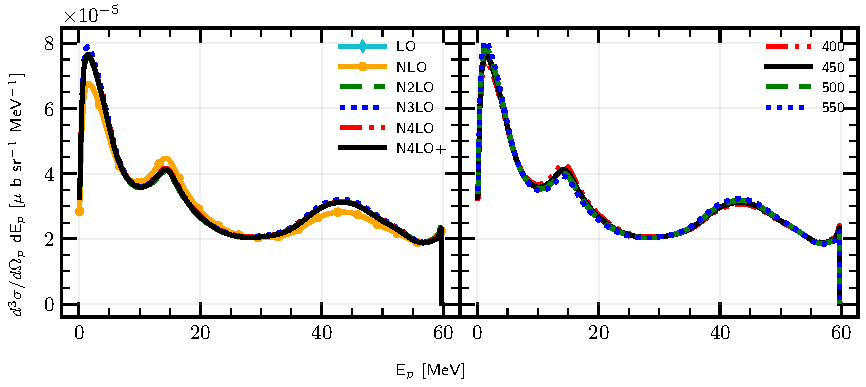
\includegraphics[width=\textwidth]{Figures_HE/CROSS_incl_100mev_90deg.pdf}
                \caption{$\theta_1 = 90^\circ$}
                \label{Diff_cross_cutoff}
            \end{subfigure}
            \begin{subfigure}[b]{0.7\textwidth}
                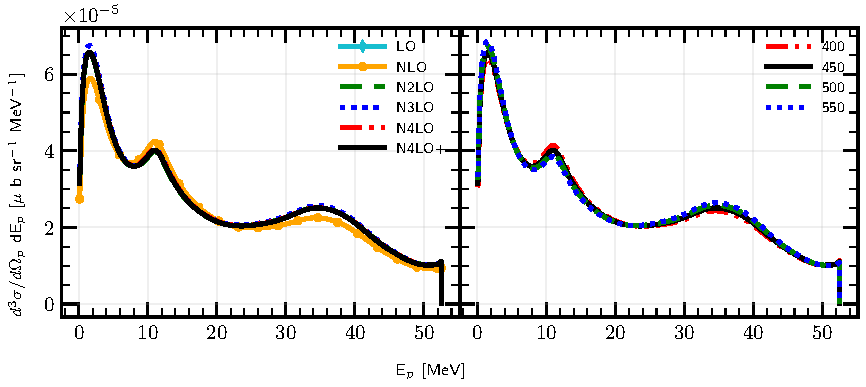
\includegraphics[width=\textwidth]{Figures_HE/CROSS_incl_100mev_130deg.pdf}
                \caption{$\theta_1 = 130^\circ$}
                \label{Diff_cross_cutoff}
            \end{subfigure}
            % \begin{subfigure}[b]{0.7\textwidth}
            %     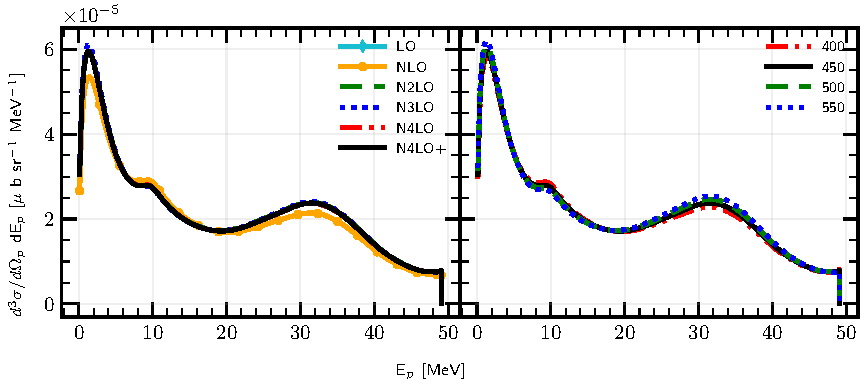
\includegraphics[width=\textwidth]{Figures_HE/CROSS_incl_100mev_170deg.pdf}
            %     \caption{Cutoff dependance}
            %     \label{Diff_cross_cutoff}
            % \end{subfigure}
            
            \caption{Inclusive cross section. E$_\gamma$=100~MeV}
        \end{figure}


\subsection{Nd photodisintegration}

\begin{figure}[h]
    \begin{center}
        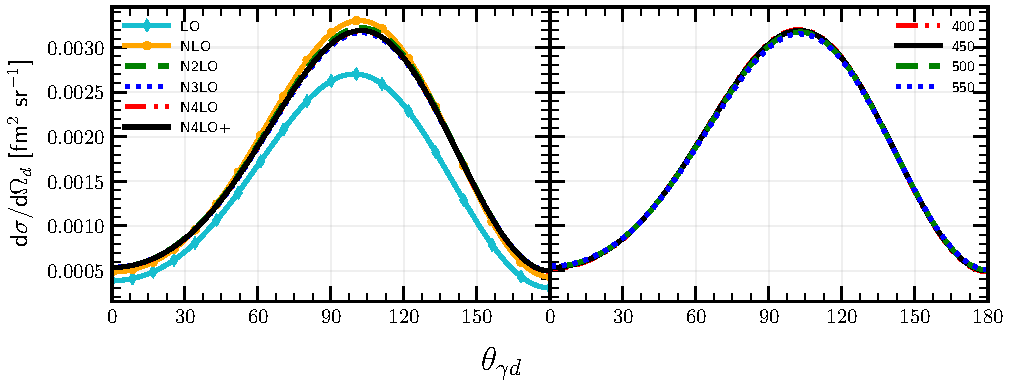
\includegraphics[width=0.9\textwidth]{Figures_HE/CROSS_nd_30mev.pdf}
        \end{center}
        \caption{Differential cross section for the d-$\gamma$ 
        two-body photodisintegraion of $^3$He as a function of the d$\gamma$ angle.
        The initial photon energy $E_\gamma=30$~MeV.}
        \label{CROSS_nd_30}
    \end{figure}


    \begin{figure}[h]
        \begin{center}
        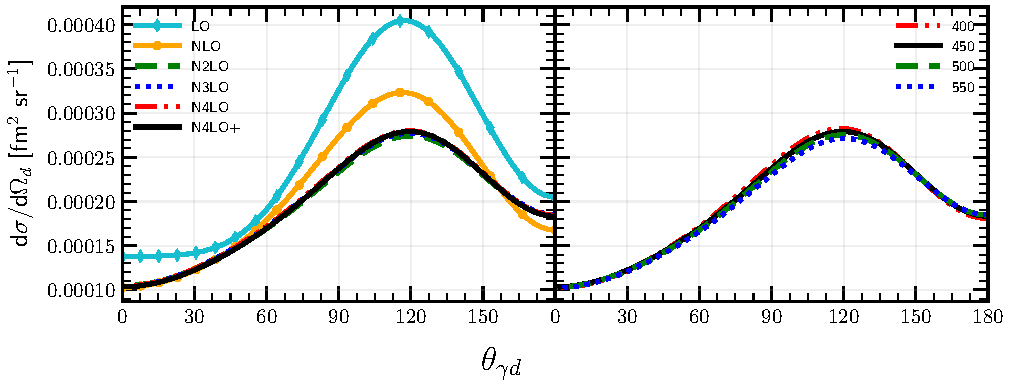
\includegraphics[width=0.9\textwidth]{Figures_HE/CROSS_nd_100mev.pdf}
        \end{center}
        \caption{The same as on Fig.~\ref{CROSS_nd_30} but 
        for the photon energy E$_\gamma=100$~MeV}
        \label{CROSS_nd_100}
    \end{figure}

